\documentclass[10pt,journal,compsoc]{IEEEtran}
% \usepackage[margin=1.3in]{geometry}
% \addtolength{\topmargin}{-.2in}
% \addtolength{\topmargin}{-.2in}
\usepackage{amssymb}
\usepackage{amsmath,amsthm}
\usepackage{url}
%\usepackage{tabularx}
\usepackage[table]{xcolor}
\usepackage{color}
\usepackage{caption}
\usepackage{algorithm}
\usepackage{algorithmicx}
% \usepackage{algorithm2e}
\usepackage{graphicx}
\usepackage{pgfplots}
\usepackage{comment}
\usepackage{mathrsfs} 
\usepackage{subcaption}
\usepackage{threeparttable}
\usepackage{multirow}
\usepackage{array}
\usepackage{mathrsfs} 
\usepackage{booktabs}

\newtheorem{Theorem}{Theorem}
\newtheorem{Definition}{Definition}
\newtheorem{Observation}{Observation}


\title{Scalable Key-Aggregate Cryptosystem for Secure Online Data Sharing on the Cloud}
\begin{document}
% 
% \author{}
% \institute{}

\author{Sikhar Patranabis, Yash Shrivastava and Debdeep Mukhopadhyay
\\Department of Computer Science and Engineering\\ Indian Institute of Technology Kharagpur
\\\{sikhar.patranabis, yash.shrivastava, debdeep\}@cse.iitkgp.ernet.in}
\maketitle
% \toctitle{Lecture Notes in Computer Science}
% \tocauthor{Authors' Instructions}


\begin{abstract}

Online data sharing for increased productivity and efficiency is one of the primary requirements today for any organization. The advent of cloud computing has pushed the limits of sharing across geographical boundaries, and has enabled a multitude of users to contribute and collaborate on shared data. However, protecting online data is critical to the success of the cloud, which leads to the requirement of efficient and secure cryptographic schemes for the same. Data owners would ideally want to store their data/files online in an encrypted manner, and delegate decryption rights for some of these to users, while retaining the power to revoke access at any point of time. An efficient solution in this regard would be one that allows users to decrypt multiple classes of data using a single key of constant size that can be efficiently broadcast to multiple users. In this paper, we address this problem by proposing  a dynamic, scalable and efficient key aggregate encryption scheme with provable security and user revocation properties. We lay special focus on how the scheme can be actually deployed on the cloud for multiple data owners and data users. We present simulation results to prove the efficiency of the scheme and compare its performance with other existing cryptosystems for online data sharing in literature.

\begin{IEEEkeywords}
 Cloud Computing, Data Sharing, Data Security, Key-Aggregate Cryptosystem, Provable Security, Scalability, Revocation
\end{IEEEkeywords}

% \noindent{\textbf{Keywords:}} Key-Aggregate Cryptoystem, Online data sharing, Semantic security, Dynamic access rights
\end{abstract}

\section{Introduction}
\label{sec:Intro}

The advent of cloud computing and the Internet of Things (IoT) has led to a massive rise in the demand for online data storage and data sharing services. Two very important paradigms that any data sharing service provider must ensure are privacy and flexibility. Since online data almost always resides in shared environments (for instance, multiple virtual machines running on the same physical device), ensuring privacy is a non trivial task. Current technology for secure data sharing comes in two major flavors - trusting a third party auditor \cite{cryptoeprint:2009:579} or using the user's own key to encrypt her data \cite{chow2012dynamic}. Figure \ref{fig:intro} describes a realistic online data sharing set-up. Suppose a data owner stores multiple classes of encrypted data online with the intention of providing users decryption keys to one or more such ciphertext classes, based on their respective credentials. She might also wish to dynamically update the delegated access rights based on 
changes to the data/credibility issues. The challenge therefore is to provide her with a secure and efficient online data sharing scheme that allows updates to user access rights on the fly. 


A n\"{a}ive (and extremely inefficient) solution is to have a different decryption key for each ciphertext class, and share them accordingly with users via secured channels. A more efficient proposition is the key-aggregate encryption (KAC) scheme proposed in \cite{chu2014key} that combines the power of individual decryption keys, for ciphertext classes in a given subset, into a single key for that subset. This key is specific to the designated subset, meaning that it cannot be used to decrypt any ciphertext class outside that subset. KAC derives its roots from the seminal work by Boneh \textit{et.al.} \cite{boneh2005collusion} that allows broadcasting of data (encrypted by the same public key) among multiple users, each of whom possess their own private keys for decryption. Both these schemes make use of bilinear mappings on multiplicative cyclic groups. 

 
 \begin{figure}[!t]
\centering
\captionsetup{font=scriptsize}
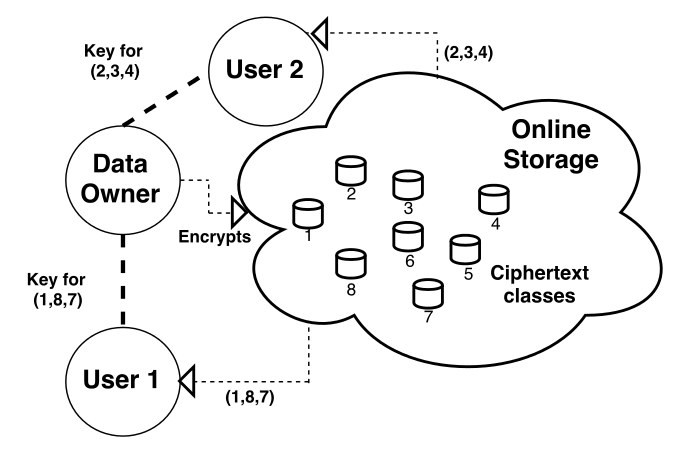
\includegraphics[scale=0.25]{Figs/KeyAgg.png}
\caption{Example of Online Data Sharing}
\label{fig:intro}
\end{figure}


\noindent{\textbf{Contributions:}} In this paper, we propose a basic key-aggregate scheme on additive elliptic subgroups that delegate decryption rights to multiple ciphertext classes using a single constant sized key. The scheme is dynamic in nature, that is, it allows the data owner to revoke access rights of users without having to change the entire set-up, unlike in the existing KAC scheme.  We then generalize this scheme into a two-level construction that allows flexible public key extension and maintains constant ciphertext size, while avoiding many of the pitfalls of earlier hierarchical schemes. We provide a formal proof of semantic security for the generalized scheme. We further extend the generalized scheme to allow using popular and efficiently implementable elliptic curve pairing schemes. We compare the time and space requirements of the proposed generalized scheme under various operating configurations. We also compare the performance of our proposed scheme, in terms of key size and resource 
utilization, with that of other existing schemes in literature.

\noindent{\textbf{Organization:}} The rest of the paper is organized as follows. Section \ref{sec:relwork} provides a brief overview of state of the art data sharing schemes. Section \ref{sec:prelims} introduces the notion of key aggregate cryptosystem, and provides a description of the complexity assumptions used to prove the semantic security of our proposed schemes. Our basic dynamic key-aggregate scheme is presented in Section \ref{sec:proposal}. We follow up with a more generalized two-tiered construction of the scheme for efficient public key extension in Section \ref{sec:general}, and prove its semantic security. A further extension for the generalized scheme that allows using efficiently implementable pairings is introduced and proved semantically secure in Section \ref{sec:extended}. Experimental results using Tate pairings based implementations of the extended scheme are presented in Section \ref{sec:results}. Finally Section \ref{sec:conclusions} concludes the paper.  



\section{Preliminaries}
\label{sec:prelims}

In this section, we formally define the key-aggregate cryptosystem~(KAC) framework as well its security. For clarity of understanding, we present the definition in two parts. The first part defines a basic KAC framework that focuses on generating small aggregate keys for arbitrarily large subsets of data classes. The second part extends this basic framework by combining it with broadcast encryption systems to distribute the aggregate key among multiple data users.

\subsection{Key-Aggregate Cryptosystem : The Basic Version}
\label{subsec:basic_framework}

The basic KAC is an ensemble of five poly-time randomized algorithms that are described next:\\

\noindent\textbf{SetUp}($\mathcal{ID}$): A data owner can classifying her data into one or more classes belonging an identity space $\mathcal{ID}$. The function sets up the key-aggregate cryptosystem for the identity space $\mathcal{ID}$. Outputs the public parameter $param$. \\

\noindent\textbf{KeyGen}(): Outputs a master-secret key $msk$ and the corresponding public key $PK$. A unique tuple $(msk,PK)$ is generated for each data owner.\\ 

\noindent\textbf{Encrypt}$(param,PK,i,\mathcal{M})$: Takes as input the public key parameter $PK$, the data class $i\in\mathcal{ID}$ and the plaintext message $\mathcal{M}$. Outputs the corresponding ciphertext $\mathcal{C}$, which is stored online in the shared environment.\\

\noindent\textbf{Extract}$(param,msk,\mathcal{S})$: Takes as input the master secret key and a polynomial size subset of data classes $\mathcal{S} \subseteq\mathcal{ID}$. Computes the aggregate key $K_{\mathcal{S}}$ for all encrypted data/messages classified into any class in $\mathcal{S}$.\\

\noindent\textbf{Decrypt}$(param,\mathcal{C},i,\mathcal{S},K_{\mathcal{S}})$: Takes as input the ciphertext $\mathcal{C}$, the data class $i$ and the aggregate key $K_{\mathcal{S}}$ corresponding to a subset $\mathcal{S}$. If $i\notin\mathcal{S}$, output $\bot$. Otherwise, outputs the decrypted message $\mathcal{M}$. The \textbf{Decrypt} function is invoked by a data user with the appropriate credentials to access one or more classes of data owned by the data owner. Note that the \textbf{Decrypt} operation for a given data user requires the explicit knowledge of the subset $\mathcal{S}$ of data classes that the corresponding user can access. This is of course a valid requirement since each user is expected to be aware of the subset $\mathcal{S}$ of data classes that she can access.

\subsubsection{Correctness.} For correctness, we require that the decryption algorithm always succeeds in decrypting a correctly encrypted plaintext message $m$. Formally, correctness of KAC may be described as follows. For any valid identity space $\mathcal{ID}$, any set $\mathcal{S}\subseteq\mathcal{ID}$, any index $i\in\mathcal{S}$, and any plaintext message $m$, we must have 
\begin{equation}
 Pr[\textbf{Decrypt}(\mathcal{C},i,\mathcal{S},K_{\mathcal{S}})=\mathcal{M} |\mathcal{E}]=1\nonumber
\end{equation}
where $\mathcal{E}$ is the event described as the conjunction of the following atomic events:
\begin{equation}
\begin{split}
param\leftarrow\textbf{SetUp}(\mathcal{ID}),(msk,PK)\leftarrow\textbf{KeyGen}(),\\
\mathcal{C}\leftarrow\textbf{Encrypt}(param,PK,i,\mathcal{M}),K_{\mathcal{S}}\leftarrow\textbf{Extract}(msk,\mathcal{S})\nonumber
\end{split} 
\end{equation}


\subsection{Security Definitions}
\label{subsec:security}

We define a formal framework for proving active chosen ciphertext security of KAC. We begin by introducing a game between a non-adaptive attack algorithm $\mathcal{A}$ and a challenger $\mathcal{B}$, both of whom are given $\mathcal{ID}$, the data class identity space, as input. The game proceeds through the following stages.\\
 
\noindent\textbf{SetUp}: Challenger $\mathcal{B}$ sets up the KAC system. In particular, $\mathcal{B}$ generates the public parameter $param$, the master secret key $msk$ and the public key $PK$. Of these, $param$ and $PK$ are furnished to $\mathcal{A}$.\\
 
\noindent\textbf{Query Phase 1}: Algorithm $\mathcal{A}$ adaptively issues decryption queries $q_1,\cdots,q_w$. Here a decryption query comprises of the tuple $(\mathcal{C},v)$, where $v\in\mathcal{ID}$ is the data class of the message encrypted as $\mathcal{C}$. The challenger has to respond a valid decryption of the ciphertext.\\
 
\noindent\textbf{Commit:} $\mathcal{A}$ adaptively commits to a set $\mathcal{S} \subset \mathcal{ID}$ of data classes that it wishes to attack. Since collusion attacks are allowed in our framework, $\mathcal{B}$ furnishes $\mathcal{A}$ with the aggregate key $K_{\overline{\mathcal{S}}}$ that allows $\mathcal{A}$ to decrypt any data class $v\notin\mathcal{S}$. Next, $\mathcal{B}$ randomly chooses a data class $i\in\mathcal{S}$ and provides it to $\mathcal{A}$.\\ 
 
\noindent\textbf{Challenge}: $\mathcal{A}$ picks at random two messages $\mathcal{M}_0$ and $\mathcal{M}_1$ from the set of possible plaintext messages and provides them to $\mathcal{B}$. To generate the challenge, $\mathcal{B}$ randomly picks $b\in\{0,1\}$, and sets the challenge to $\mathcal{A}$ as $(\mathcal{C}^{*},\mathcal{M}_0,\mathcal{M}_1)$, where ${\mathcal{C}}^{*}$ = \textbf{Encrypt}($PK,i,\mathcal{M}_b$).\\
 
\noindent\textbf{Query Phase 2}: $\mathcal{A}$ continues to adaptively issue decryption queries $q_{w+1},\cdots,q_{Q_D}$ where a decryption query comprises of the tuple $(\mathcal{C},v)$, but is now subject to the restriction $\mathcal{C}\neq {\mathcal{C}}^{*}$. $\mathcal{B}$ responds as in query phase 1.\\ 
 
 
\noindent\textbf{Guess}: $\mathcal{A}$ outputs a guess $b'$ of $b$. If $b' = b$, $\mathcal{A}$ wins the game.\\

% Note that the adversary $\mathcal{A}$ is non-adaptive; it chooses $\mathcal{S}$, and obtains the aggregate decryption key for all data classes outside of $\mathcal{S}$, before it even sees the public parameters $param$ or the public key $PK$

% \vspace{-2mm}
\noindent The game above models an attack in the real world setting where users who do not have authorized access to the subset $\mathcal{S}$ collude to try and expose a message in this subset. We now formally define the security notions for KAC. Let $Adv_{\mathcal{A},|\mathcal{ID}|}$ denote the probability that $\mathcal{A}$ wins the game.
\subsubsection{Definition 2.1.}
 A KAC construction is $(\epsilon,\mathcal{ID},Q_D)$ adaptively secure under a chosen ciphertext attack (that is, adaptively CCA-secure) if, for all adaptive probabilistic ploy-time algorithms $\mathcal{A}$ that can make a total of $Q_D$ decryption queries, we have that $|Adv_{\mathcal{A},|\mathcal{ID}|}-\frac{1}{2}| < \epsilon$.
 
\subsubsection{Definition 2.2.}
 A KAC construction is $(\epsilon,\mathcal{ID})$ adaptively secure under a chosen plaintext attack (that is, adaptively CPA-secure) if it is $(\epsilon,\mathcal{ID},0)$ adaptively CCA secure.\\


\noindent We also define two weaker notions of security in the non-adaptive setting. In particular, non-adaptive security is achieved in the scenario when $\mathcal{A}$ is required to commit to the set $\mathcal{S}$ before seeing the public parameters. We refer to such an adversary as a non-adaptive adversary. This leads to the following definitions.

\subsubsection{Definition 2.3.}
 A KAC construction is $(\epsilon,\mathcal{ID},Q_D)$ non-adaptively secure under a chosen ciphertext attack (that is, non-adaptively CCA-secure) if, for all non-adaptive probabilistic ploy-time algorithms $\mathcal{A}$ that can make a total of $Q_D$ decryption queries, we have that $|Adv_{\mathcal{A},|\mathcal{ID}|}-\frac{1}{2}| < \epsilon$.
% \end{Definition}

\subsubsection{Definition 2.4.}
 A KAC construction is $(\epsilon,\mathcal{ID})$ non-adaptively secure under a chosen plaintext attack (that is, non-adaptively CPA-secure) if it is $(\epsilon,\mathcal{ID},0)$ non-adaptively CCA secure.
% \end{Definition}

\subsection{Extensions to The Basic Version : Broadcasting Aggregate Keys}
\label{subsec:extensions}

We discuss in this paper two extensions to the basic framework of KAC for a full-fledged public key based implementation in practical data sharing environments. We first note that the standalone KAC framework presented in Section \ref{subsec:basic_framework} is a perfectly suitable choice when a single data owner wishes to delegate access rights to a particular subset of her data to a given data user. However, any practically deployable online data sharing scheme must be able to support multiple data owners, who should in turn be able to delegate access rights to their data to multiple users. In this context, there are two major requirements that the standalone KAC framework does not explicitly cater to:

\begin{itemize}
 \item Data privacy must be ensured for each individual data owner. In particular, an aggregate decryption key issued by one data owner should not leak information about the data of another data owner to an unauthorized user.
 \item Distribution of aggregate keys to a large number of data users must be handled efficiently and, preferably, via a public key based protocol and not a secure channel as suggested in \cite{chu2014key}.
\end{itemize}

\noindent In this paper, we augment the basic KAC framework to tackle both these problems efficiently. In particular, the second problem is handled by combining the basic KAC framework with that of the identity-based broadcast encryption scheme proposed in \cite{boneh2014low}. We formally define the combined scheme, referred to as the \emph{extended} KAC framework, using the following set of algorithms. Note that $\mathcal{ID}_1$ and $\mathcal{ID}_2$ denote the identity spaces for the data classes and the data users respectively.\\

\noindent\textbf{SetUp}($\mathcal{ID}_1,\mathcal{ID}_2$): Same as the basic KAC framework. \\

\noindent\textbf{OwnerKeyGen}(): In addition to the public key $PK$ and the master-secret key $msk$, also outputs a distribution-secret key $dsk$. The tuple $(msk,PK,dsk)$ is made available to the data owner.\\ 

\noindent\textbf{Encrypt}$(param,PK,dsk,i,\mathcal{M})$: Takes as input the data class $i\in\mathcal{ID}_1$ and the plaintext message $\mathcal{M}$. Outputs the corresponding ciphertext $\mathcal{C}$.\\

\noindent\textbf{UserKeyGen}$(param,msk,\hat{i})$: Takes as input the index $\hat{i}\in\mathcal{ID}_2$ for a user and outputs the corresponding secret key $d_{\hat{i}}$.\\ 

\noindent\textbf{Extract}$(param,msk,\mathcal{S})$: Takes as input the master secret key and a polynomial size subset of data classes $\mathcal{S} \subseteq\mathcal{ID}_1$. Computes the aggregate key $K_{\mathcal{S}}$ for all encrypted data/messages classified into any class in $\mathcal{S}$.\\

\noindent\textbf{Broadcast}$(param,K_{\mathcal{S}},\hat{\mathcal{S}},PK,dsk)$: Takes as input the aggregate key $K_{\mathcal{S}}$, the polynomial size target subset of users $\hat{\mathcal{S}}\subseteq\mathcal{ID}_2$. Outputs a single \emph{broadcast aggregate key} $K_{\left(\mathcal{S},\hat{\mathcal{S}}\right)}$ that allows any user $\hat{i}\in\hat{\mathcal{S}}$ to decrypt all encrypted data/messages classified into any class $i\in\mathcal{S}$.\\

\noindent\textbf{Decrypt}$(param,\mathcal{C},K_{\left(\mathcal{S},\hat{\mathcal{S}}\right)},i,\hat{i},d_{\hat{i}},\mathcal{S},\hat{\mathcal{S}})$: The decryption algorithm now takes, besides the ciphertext $\mathcal{C}$ and the corresponding data class $i\in\mathcal{S}$, a valid user id $\hat{i}\in\hat{\mathcal{S}}$. It also takes as input the broadcast aggregate key $K_{\left(\mathcal{S},\hat{\mathcal{S}}\right)}$ and the secret key $d_{\hat{i}}$. The algorithm outputs the decrypted message.\\

% \noindent We avoid presenting separately the game-based security framework for the extended KAC scheme here. The framework is directly introduced when proving the security of our proposed construction in Section \ref{subsec:multiuserKAC}.

\subsection{Security of Extended KAC: A Game Based Framework}
\label{subsec:gameextended}

We also define the formal framework for proving the security of the extended KAC via the following game between an attack algorithm $\mathcal{A}$ and a challenger $\mathcal{B}$:\\

\noindent\textbf{SetUp}: Challenger $\mathcal{B}$ sets up the KAC system. In particular, $\mathcal{B}$ generates the public parameter $param$, the master secret key $msk$, the distribution secret key $dsk$ and the public key $PK$. Of these, $param$ and $PK$ are furnished to $\mathcal{A}$.\\
 
\noindent\textbf{Query Phase 1}: Algorithm $\mathcal{A}$ adaptively issues decryption queries $q_1,\cdots,q_w$. Here a decryption query comprises of the tuple $(\mathcal{C},v)$, where $v\in\mathcal{ID}$ is the data class of the message encrypted as $\mathcal{C}$. The challenger has to respond a valid decryption of the ciphertext.\\
 
\noindent\textbf{Commit:} $\mathcal{A}$ adaptively commits to a set $\mathcal{S} \subset \mathcal{ID}_1$ of data classes and a corresponding set $\hat{\mathcal{S}} \subset \mathcal{ID}_2$ of authorized data users (with access to $\mathcal{S}$) that it wishes to attack. Since collusion attacks are allowed in our framework, $\mathcal{B}$ furnishes $\mathcal{A}$ with all the private user keys $d_{\hat{j}}$ for $\hat{j}\notin\hat{\mathcal{S}}$. In addition, $\mathcal{A}$ is also provided with the broadcast aggregate key $K_{\left(\overline{\mathcal{S}},\hat{\mathcal{S}}\right)}$ that allows any user in $\hat{\mathcal{S}}$ to decrypt any ciphertext class $v\notin{\mathcal{S}}$.\\  
 
\noindent\textbf{Challenge}: $\mathcal{A}$ picks at random two messages $\mathcal{M}_0$ and $\mathcal{M}_1$ from the set of possible plaintext messages and provides them to $\mathcal{B}$. To generate the challenge, $\mathcal{B}$ randomly picks $b\in\{0,1\}$, and sets the challenge to $\mathcal{A}$ as $(\mathcal{C}^{*},\mathcal{M}_0,\mathcal{M}_1)$, where ${\mathcal{C}}^{*}$ = \textbf{Encrypt}($PK,i,\mathcal{M}_b$).\\
 
\noindent\textbf{Query Phase 2}: $\mathcal{A}$ continues to adaptively issue decryption queries $q_{w+1},\cdots,q_{Q_D}$ where a decryption query comprises of the tuple $(\mathcal{C},v)$, but is now subject to the restriction $\mathcal{C}\neq {\mathcal{C}}^{*}$. $\mathcal{B}$ responds as in query phase 1.\\

\noindent\textbf{Guess}: $\mathcal{A}$ outputs a guess $b'$ of $b$. If $b' = b$, $\mathcal{A}$ wins the game.\\

The game above models an attack involving two different kinds of collusion. The first collusion is by all users not in $\hat{\mathcal{S}}$ who collude to try and expose an aggregate key that is broadcast for users in $\hat{\mathcal{S}}$ only. The second collusion is by users in $\hat{\mathcal{S}}$ who collude (by compromising the knowledge of the aggregate key for different subsets) to try and expose a message class in $\mathcal{S}$.

We next define the security of extended KAC. Let $Adv'_{\mathcal{A},|\mathcal{ID}_1|,|\mathcal{ID}_2|}$ denote the probability that $\mathcal{A}$ wins the above game.

\subsubsection{Definition 2.5.}
An extended KAC construction with the ability to broadcast aggregate keys is $(\epsilon,mathcal{ID}_1,\mathcal{ID}_2,Q_D)$ non-adaptively secure under a chosen ciphertext attack (that is, non-adaptively CCA-secure) if, for all non-adaptive probabilistic ploy-time algorithms $\mathcal{A}$ that can make a total of $Q_D$ decryption queries, we have that $|Adv'_{\mathcal{A},|\mathcal{ID}_1|,|\mathcal{ID}_2|}-\frac{1}{2}| < \epsilon$.
% \end{Definition}

\subsubsection{Definition 2.6.}
An extended KAC construction is $(\epsilon,\mathcal{ID}_1,\mathcal{ID}_2)$ non-adaptively secure under a chosen plaintext attack (that is, non-adaptively CPA-secure) if it is $(\epsilon,\mathcal{ID}_1,\mathcal{ID}_2,0)$ non-adaptively CCA secure.
 

\subsection{Multilinear Maps}
\label{subsec:multilinear}

In this section, we provide a brief overview of multilinear maps. Our description of multilinear maps is based on the \emph{graded encoding scheme} used in several candidate multilinear map constructions \cite{garg2013candidate}.

\subsubsection{Symmetric Multilinear Maps.} A standard symmetric multilinear map consists of the following pair of algorithms.\\

\noindent\textbf{SetUp}$'(1^\lambda,m)$: Sets up an $m$-linear map by outputting an $m$-tuple of groups $<\mathbb{G}_1,\mathbb{G}_2,\cdots,\mathbb{G}_m>$ of prime order $q$ (where $q$ is a $\lambda$ bit prime), along with the respective generator $g_i\in\mathbb{G}_i$ for $1\leq i\leq m$. In standard notation, $\mathbb{G}_1$ is the source group, $\mathbb{G}_m$ is the target group, and $\mathbb{G}_2,\cdots,\mathbb{G}_{m-1}$ are the intermediate groups.\\

\noindent$e_{i,j}(h_1,h_2)$: Takes as input $h_1\in\mathbb{G}_i$ and $h_2\in\mathbb{G}_j$, and outputs $h_3\in\mathbb{G}_{i+j}$ such that
\begin{equation}
 (h_1=g_i^a,h_2=g_j^b) \Rightarrow h_3=g_{i+j}^{ab}\nonumber
\end{equation}
\noindent In this paper, we follow the standard notation used in the literature to omit the subscripts and simply refer to this multilinear map as $e$. Further, $e$ may be generalized to multiple inputs as $e(h_1,\cdots,h_k)=e(h_1,e(h_2,\cdots,h_k))$. Note that $g^a_i$ is sometimes referred to as the level-$i$ \emph{encoding} of $a$. The scalar $a$ itself may therefore be referred to as the level $0$ encoding of itself.

\subsubsection{Asymmetric Multilinear Maps.} We adopt the same definition of asymmetric multilinear maps presented in \cite{garg2013candidate}. According to this definition, in asymmetric multilinear maps, the groups are indexed by integer vectors. Formally, a standard asymmetric multilinear map consists of the following algorithms.\\

\noindent\textbf{SetUp}$''(1^\lambda,\mathbf{m})$: Takes as input $\mathbf{m}\in\mathbb{Z}^l$. Sets up an $\mathbf{m}$-linear map by outputting an $m$-tuple of groups $<\mathbb{G}_{\mathbf{1}},\mathbb{G}_{\mathbf{2}},\cdots,\mathbb{G}_{\mathbf{m}}>$ of prime order $q$ (where $q$ is a $\lambda$ bit prime), along with the respective generator $g_{\mathbf{v}}\in\mathbb{G}_{\mathbf{v}}$ for $\mathbf{1}\leq \mathbf{v}\leq \mathbf{m}$(comparison is defined component-wise). Further, let $\mathbf{x}_i$ be the $i$th \emph{standard} basis vector (with $1$ at position $i$ and $0$ at each other position). In standard notation, $\mathbb{G}_{\mathbf{x}_i}$ is the $i$th source group, $\mathbb{G}_{\mathbf{v}}$ is the target group, and the rest are the intermediate groups.\\

\noindent$e_{\mathbf{i},\mathbf{j}}(h_1,h_2)$: Takes as input $h_1\in\mathbb{G}_\mathbf{i}$ and $h_2\in\mathbb{G}_\mathbf{j}$, and outputs $h_3\in\mathbb{G}_\mathbf{i+j}$ such that
\begin{equation}
 (h_1=g_\mathbf{i}^a,h_2=g_\mathbf{j}^b)\Rightarrow h_3=g_\mathbf{i+j}^{ab}\nonumber
\end{equation}
\noindent Again, we omit the subscripts and simply refer to this multilinear map as $e$, which may be generalized to multiple inputs as $e(h_1,\cdots,h_k)=e(h_1,e(h_2,\cdots,h_k))$.\\ 

In the forthcoming discussions, we present our KAC constructions assuming that the ideal multilinear maps based on the graded encoding scheme described above exist and are efficiently computable. We do this to make the analysis simple and easy to follow. We point out, however, that current candidates for multilinear maps in the cryptographic literature deviate from these ideal notions. In these candidates, group elements lack unique representations due to the presence of a noise term that tends to grow with repeated group/multilinear operations. However, as pointed out in \cite{boneh2014low}, most candidate constructions \cite{garg2013candidate,coron2013practical,gentry2014zeroizing,boneh2014immunizing} possess the necessary properties to instantiate public key constructions based on ideal multilinear maps. Unfortunately, most of these constructions have been cryptanalyzed \cite{cheon2015cryptanalysis,coron2014cryptanalysis}. To the best of our knowledge, the foremost candidate construction for multilinear maps currently unbroken is the graph-induced multilinear map based on lattices proposed by Gentry et al. \cite{gentry2015graph}, which naturally gives rise to asymmetric multilinear maps. We point out that it is possible to instantiate our KAC constructions using this candidate map since it meets our requirements listed below:

\let\labelitemi\labelitemii

\begin{itemize}
 \item The representation of an element should be statistically independent of the group and multilinear operations that led to that element. This is achieved using Kilian-style randomization \cite{kilian1988founding} on the encoding side \cite{gentry2015graph}.\\
 \item It is possible to extract a \emph{canonical} representation of an element in the target group given any representation of that element using the \emph{zero-test parameter}.\\
 \item The party setting up the multilinear map has sufficient \emph{trapdoor} information to compute $g^{\alpha^x}$ for a non-random $\alpha$ and exponentially large $x$.\\
 \item It is possible to generate asymmetric multilinear maps for any positive integer vector $\mathbf{m}\in\mathbb{Z}^l$.\\
%  \item It should be possible to design the parameters of our system such that the noise growth during the execution of our scheme does not lead to erroneous computations. 
\end{itemize}

\noindent However, in order to successfully instantiate our proposed schemes using graph induced multilinear map candidates, it is important to ensure that the algebraic elements used in our constructions are suitably encoded as paths in a directed graph and adequate precautions are taken to prevent weak trapdoor attacks.  

% We point out that the two foremost candidates for multilinear maps based on graded encoding schemes - the GGH candidate over ideal lattices \cite{garg2013candidate} and the CLT candidate over integers \cite{coron2013practical} would allow us to meet all these requirements. However, we also note that both these candidate constructions have been subjected to \emph{zeroizing attacks}\cite{cheon2015cryptanalysis}, also known as the weak discrete logarithmic attack. These attacks break the Subgroup Membership (SubM) and the decision linear (DLIN) problems on the GGH candidate map, and also completely break the CLT candidate. Initially it was conjectured that this attack could be thwarted by keeping the low-level encodings of $0$ private in the candidate constructions, and several fixes to these candidate constructions were provided based on this idea \cite{gentry2014zeroizing,boneh2014immunizing}. However, these extensions were also proven to be insecure in \cite{coron2014cryptanalysis}. 
% 
% In this paper, we propose using use the graph-induced multilinear map based on lattices proposed by Gentry et al. \cite{gentry2015graph} to instantiate our constructions. The graph-induced multilinear map, like the GGH and CLT candidate constructions, is also based on the graded encoding scheme and meets almost all the requirements listed above. The only significant drawback of this construction is the absence of the \emph{re-randomization} procedure (that helps to hide the group and multilinear operations leading to a particular element) to thwart cryptanalytic threats. However, a work around suggested in \cite{gentry2015graph} is to use Kilian-style randomization \cite{kilian1988founding} on the encoding side. This enhances the security of any scheme based on the graph induced candidate map, at the cost of some extra encoding bits.




% \noindent\textbf{The Multilinear Diffie-Hellman Exponent (MDHE) Assumption}:  Let $param\leftarrow SetUp'(n+l-1)$. Choose random 


 









\section{The Proposed Dynamic Key-Aggregate Cryptosystem: The Basic Case}
\label{sec:proposal}

In this section, we present the design of our proposed dynamic key-aggregate storage scheme on additive elliptic curve subgroups assuming that there are $n$ ciphertext classes. Our scheme ensures that the ciphertext and aggregate key are of constant size, while the public parameter size is linear in the number of ciphertext classes. Unlike the scheme proposed in \cite{chu2014key}, the proposed scheme allows dynamic revocation of user access rights without having to massively change the system parameters. We also present a proof of security for the proposed scheme.

\subsection{The Basic Construction of Dynamic KAC}
\label{subsec:construction1}

Let $\mathbb{G}$ be an additive cyclic elliptic curve subgroup of prime order $q$, where $2^{\lambda}\leq q \leq 2^{\lambda + 1}$, such that the point $P$ is a generator for $\mathbb{G}$. Also, let $\mathbb{G}_{T}$ be a multiplicative group of order $q$ with identity element $1$. We assume that there exists an efficiently computable bilinear pairing $\hat{e'}:\mathbb{G} \times \mathbb{G}\longrightarrow\mathbb{G}_T$. We now present the basic construction of our proposed key-aggregate encryption scheme. 

The scheme consists of the following five phases.

\begin{enumerate}
 \item \textbf{Setup}$(1^{\lambda},n)$: Randomly pick $\alpha \in \mathbb{Z}_q$. Compute $P_i = {\alpha^{i}}P \in \mathbb{G}$ for $i = 1,\cdots,n,n+2,\cdots,2n$. Output the system parameter as\\
 $param = (P,P_1,\cdots,P_n,P_{n+2},\cdots,P_{2n})$. The system also randomly chooses a secret parameter $t \in \mathbb{Z}_q$ which is not made public. It is only known to data owners with credentials to control client access rights.
 \item \textbf{Keygen}(): Pick $\gamma \in \mathbb{Z}_q$, output the public and master-secret key pair : \\$(PK={\gamma}P,msk=\gamma)$.
 \item \textbf{Encrypt}$(PK,i,m)$: For a message $m \in \mathbb{G}_T$ and an index $i \in \{1,2,\cdots,n\}$, randomly choose $r\in\mathbb{Z}_q$ and let $t'=t+r \in\mathbb{Z}_q$. Then the ciphertext is computed as\\ $\mathcal{C}=(rP,t'{(PK+P_i)},m.\hat{e'}(P_n,t'P_1))$ $=$ $(c_1,c_2,c_3)$
 \item \textbf{Extract}$(msk=\gamma,\mathcal{S})$: For the set $\mathcal{S}$ of indices $j$ the aggregate key is computed as\\ $K_{\mathcal{S}} = \sum_{j\in\mathcal{S}}{\gamma}P_{n+1-j}$ = $\sum_{j\in\mathcal{S}}\alpha^{n+1-j}PK$\\ and the dynamic access control parameter $U$ is computed as $tP$. Thus the net aggregate key is $(K_{\mathcal{S}},U)$ which is transmitted via a secure channel to users that have access rights to $\mathbb{S}$.
 \item \textbf{Decrypt}$(K_{\mathcal{S}}, U, \mathcal{S},i,\mathcal{C}=\{c_1,c_2,c_3\})$: If $i\notin\mathcal{S}$, output $\bot$. Otherwise return the message\\ $\hat{m}=c_3\hat{e'}(K_{\mathcal{S}}+\sum_{j\in\mathcal{S},j\neq i}P_{n+1-j+i},U+c_1)/(\hat{e'}(\sum_{j\in\mathcal{S}}P_{n+1-j},c_2))$. 
\end{enumerate}

The proof of correctness of this scheme is presented below.

\begin{scriptsize}
\begin{equation*}
\label{eq:correctness}
\begin{split}
 \hat{m} &= c_3\frac{\hat{e'}(K_{\mathcal{S}}+\sum_{j\in\mathcal{S},j\neq i}P_{n+1-j+i},U+c_1)}{\hat{e'}(\sum_{j\in\mathcal{S}}P_{n+1-j},c_2)}\\
%   &= c_3\frac{\hat{e'}(\sum_{j\in \mathcal{S}}{\gamma}P_{n+1-j} + \sum_{j\in\mathcal{S},j\neq i}P_{n+1-j+i},t'P)}{\hat{e'}(\sum_{j\in\mathcal{S}}P_{n+1-j},t'(PK+P_i))}\\
  &= c_3\frac{\hat{e'}(\sum_{j\in \mathcal{S}}{\gamma}P_{n+1-j},t'P)\hat{e'}(\sum_{j\in\mathcal{S}}(P_{n+1-j+i})-P_{n+1},t'P)}{\hat{e'}(\sum_{j\in\mathcal{S}}P_{n+1-j},t'PK)\hat{e'}(\sum_{j\in\mathcal{S}}P_{n+1-j},t'P_i))}\\
%   &= c_3\frac{\hat{e'}(\sum_{j\in\mathcal{S}}P_{n+1-j+i},t'P)}{\hat{e'}(P_{n+1},t'P)\hat{e'}(\sum_{j\in\mathcal{S}}P_{n+1-j},t'P_i))}\\
  &= c_3\frac{\hat{e'}(\sum_{j\in\mathcal{S}}P_{n+1-j+i},t'P)}{\hat{e'}(P_{n+1},t'P)\hat{e'}(\sum_{j\in\mathcal{S}}P_{n+1-j+i},t'P))}\\
%   &= m\frac{\hat{e'}(P_n,t'P_1)}{\hat{e'}(P_{n+1},t'P)}\\
  &= m
\end{split}  
\end{equation*}
\end{scriptsize}


\subsection{Dynamic Access Control}
\label{subsec:dynamic}

An important aspect of the proposed scheme is the fact that it allows the data owner to dynamically update user access permissions. In KAC \cite{chu2014key}, once the data owner issues an aggregate key corresponding to a set of ciphertext classes to a user, revoking the user's access permissions to the same is not possible without changing the master secret key. However, changing the master secret key each time an user's access privileges to a ciphertext class need to be updated, is a very expensive option and may not be practically feasible. Our scheme, on the other hand, offers a solution to this problem by allowing the data owner to dynamically update user access privileges.

We achieve this by making the parameter $U=tP$ a part of the aggregate key in our proposed scheme and not a part of the ciphertext. The user must have the correct value of $U$ in possession to be able to decrypt any encrypted ciphertext class in the subset $\mathcal{S}$. Now suppose the data owner wishes to alter the access rights to the subset $\mathcal{S}$. She can simply re-encrypt all ciphertexts in that class using a different random element $\hat{t}\in\mathbb{Z}_q$, and then provide the updated dynamic access parameter $\hat{U}=\hat{t}P$ to only those users who she wishes to delegate access to. The decrypted value will give the correct message $m$ only if the same $t$ is used for both encryption and decryption. This is a major difference between our scheme and the scheme proposed in \cite{chu2014key}, where the knowledge of the random parameter was only embedded as part of the ciphertext itself, and could not be used to control access rights of users. Moreover, since $U$ is of constant size and needs to be transmitted only when changed (and not for every encryption), there is no significant degradation in performance.

\subsection{Performance and Efficiency}
\label{subsec:perf}
The decryption time for any subset of ciphertext classes $\mathcal{S}$ is essentially dominated by the computation of $W_{\mathcal{S}}=\sum_{j\in\mathcal{S}}P_{n+1-j+i}$. However, if a user has already computed $\sum_{j\in\mathcal{S}'}P_{n+1-j+i}$ for a subset $S'$ similar to $S$, then she can easily compute the desired value by at most $|\mathcal{S}-\mathcal{S}'|$ operations. For similar subsets $S$ and $S'$, this value is expected to be fairly small. A suggested in \cite{boneh2005collusion}, for subsets of very large size($n-r, r\ll n$), an advantageous approach could be to pre-compute $\sum_{j=1}^{j=n}P_{n+1-j+i}$ corresponding to $i=1$ to $n$, which would allow the user to decrypt using only $r$ group operations, and would require only $r$ elements of $param$. Similar optimizations would also hold for the encryption operation where pre-computation of  $\sum_{j=1}^{j=n}P_{n+1-j}$ is useful for large subsets.

It is important to note that our proposed scheme fixes the number of ciphertext classes beforehand, thus limiting the scope for ciphertext class extension. The only way to increase the number of classes is to change the public key parameters, which would therefore require some kind of administrative privileges, and cannot be done by an user for her own purposes. However, in online data sharing environments, users may wish to register their own public key-private key pairs for new ciphertext classes according to their own requirements. Such an extension to the scheme would make extremely convenient and attractive to potential users. A proposal made in \cite{chu2014key} recommends that the user be allowed to register new public-private key pairs, at the cost of increasing the number of ciphertext classes by $n$ each time. This is both impractical and wasteful. In the next section, we present a two-tier generalization of our scheme that tackles this issue in a more economical fashion. We avoid a separate proof of semantic security for the base case presented here, since the proof is a special case of the proof for the generalized scheme presented in the next section.  
  



\section{Experimental Results Using Tate pairings}
\label{sec:results}

In this section we present experimental results from our implementations of the extended generalized scheme using Tate pairings on BN-curves using $256$ bit primes \cite{ghosh2013secure}. All our experiments have been carried out on an AMD Opteron (TM) Processor $6272\times16$ with a clock frequency $1.4$ GHz. The details of our implementations of Tate Pairings are summarized in Appendix \ref{app_sec:implementation}.

\subsection{Space and Time Complexities}

\begin{table}[!t]
\centering
\captionsetup{font=scriptsize}
\caption{Space Complexities}
\label{tab:space}
\scalebox{0.6}{
\begin{tabular}{|c|c|c|c|c|c|c|c|}
  \hline 
  $n_1$ & $n_2$ & $param$ & $PK$ & $msk$ & $K_{\mathcal{S}}$ & $U$ & Total\\
  & & (in bytes) & (in bytes) & (in bytes) & (in bytes) & (in bytes) & (in KB)\\\hline\hline
  1 & 100 & 16112 & 144 & 40 & 72 & 64 & 16.046875\\\hline
  2 & 50 & 8112 & 240 & 56 & 120 & 64 & 8.390625\\\hline
  4 & 25 & 4112 & 432 & 88 & 216 & 64 & 4.796875\\\hline
  5 & 20 & 3312 & 528 & 104 & 264 & 64 & 4.171875\\\hline
  \textbf{10} & \textbf{10} & \textbf{1712} & \textbf{1008} & \textbf{184} & \textbf{504} & \textbf{64} & \textbf{3.390625}\\\hline
  20 & 5 & 912 & 1968 & 344 & 984 & 64 & 4.171875\\\hline
  25 & 4 & 752 & 2448 & 424 & 1224 & 64 & 4.796875\\\hline
  50 & 2 & 432 & 4848 & 824 & 2424 & 64 & 8.390625\\\hline
  100 & 1 & 272 & 9648 & 1624 & 4824 & 64 & 16.046875\\\hline
  \hline
\end{tabular}}
\end{table}

\begin{table}[!t]
\centering
\captionsetup{font=scriptsize}
\caption{Time Complexities}
\label{tab:time}
\scalebox{0.6}{
% \begin{tabular}{|c|c|c|c|c|c|}
\begin{tabular}{|c|c|c|c|c|c|c|c|}
  \hline 
  $n_1$ & $n_2$ & $SetUp$ & $KeyGen$ & $Encrypt$ & $Extract$ & $Decrypt$ & Total\\
  & & (in clock cycles) & (in clock cycles) & (in clock cycles) & (in clock cycles) & (in clock cycles) & (in clock cycles)\\\hline\hline
  1 & 100 & 2920000 & 10000 & 7932000 & 47000 & 16095000 & 27004100\\\hline 
  2 & 50 & 1410000 & 30000 & 8065000 & 53000 & 16110000 & 25668000\\\hline
  4 & 25 & 690000 & 60000 & 8130000 & 81000 & 16284000 & 25245000\\\hline
  5 & 20 & 590000 & 70000 & 8091000 & 96000 & 16379000 & 25226000\\\hline
  \textbf{10} & \textbf{10} & \textbf{280000} & \textbf{140000} & \textbf{7957000} & \textbf{170000} & \textbf{16049000} & \textbf{25136000}\\\hline
  20 & 	5 & 130000 & 270000 & 8070000 & 320000 & 16361000 & 25151000\\\hline
  25 & 4 & 120000 & 350000 & 8256000 & 370000 & 16239000 & 25836000\\\hline
  50 & 2 & 50000 & 680000 & 8265000 & 712000 & 16398000 & 26105000\\\hline
  100 & 1 & 30000 & 1360000 & 8201000 & 1315000 & 16142000 & 27048000\\\hline

  \hline
\end{tabular}}
\end{table}
% \vspace{-2mm}

Table \ref{tab:space} summarizes the space requirements for various parameters of the scheme for different values of $(n_1,n_2)$. The results have been averaged over $100$ randomly chosen subsets of the $n=100$ ciphertext classes. Table \ref{tab:time} summarizes the time complexity for various operations of the scheme for different values of $(n_1,n_2)$. The results have been averaged over $100$ randomly chosen subsets of the $n=100$ ciphertext classes. The encryption and decryption operation complexities are further averaged over $10$ message transmissions corresponding to each subset. We point out that both the overall space and time requirements are minimum for $n_1=n_2=10=\surd n$, which proves the usefulnesss of the generaalization.

\subsection{Comparison with Hierarchy Based Schemes}
% \vspace{-2mm}
\begin{figure*}[!t]
\captionsetup{font=scriptsize}
\centering
% \caption{Simulation results}

% n_1:n_2	0.1	0.2	0.3	0.4	0.5	0.6	0.7	0.8	0.9
% 1:100	0.1	0.05	0.0333333	0.025	0.02	0.0166667	0.0142857	0.0125	0.0111111
% 2:50	0.2	0.1	0.0666667	0.05	0.04	0.0333333	0.0285714	0.025	0.0222222
% 4:25	0.37	0.2	0.133333	0.1	0.08	0.0666667	0.0571429	0.05	0.0497512
% 5:20	0.46	0.245	0.166667	0.125	0.1	0.0833333	0.0714286	0.0640205	0.0685871
% 10:10	0.69	0.465	0.323333	0.245	0.2	0.166667	0.150602	0.135685	0.179211
% 20:5	0.82	0.66	0.57	0.467172	0.419565	0.367647	0.34965	0.340136	0.454545
% 25:4	0.9	0.715736	0.656566	0.578534	0.5141	0.481928	0.476654	0.497018	0.617284
% 50:2	1	1	1	1	1	1	1	1	1
% 100:1	1	1	1	1	1	1	1	1	1

\begin{subfigure}{0.5\textwidth}
\captionsetup{font=scriptsize}
\centering
% \hspace*{-2.13 cm}
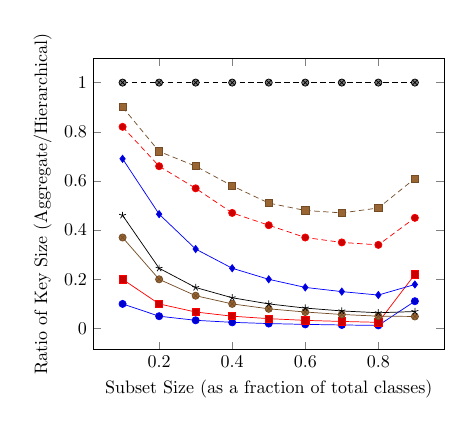
\begin{tikzpicture}[scale = 0.65]
	 \begin{axis}[
	 		xlabel=Subset Size (as a fraction of total classes),
	 		ylabel=Ratio of Key Size (Aggregate/Hierarchical),
% 	 		nolegend
	 		legend pos={north west}
	 		]
	 \addplot plot coordinates{
	 	(0.1,0.1)
		(0.2,0.05)
		(0.3,0.0333)
		(0.4,0.025)
		(0.5,0.02)
		(0.6,0.0167)
		(0.7,0.0143)
		(0.8,0.0125)
		(0.9,0.111)
	 };
	 %\addlegendentry{$n_1=1$, $n_2=100$}
	 \addplot plot coordinates{
	 	(0.1,0.2)
		(0.2,0.1)
		(0.3,0.067)
		(0.4,0.05)
		(0.5,0.04)
		(0.6,0.033)
		(0.7,0.0287)
		(0.8,0.025)
		(0.9,0.22)
	 };
	 %\addlegendentry{$n_1=2$, $n_2=50$}
	 \addplot plot coordinates{
% 	 0.37	0.2	0.133333	0.1	0.08	0.0666667	0.0571429	0.05	0.0497512
	 	(0.1,0.37)
		(0.2,0.2)
		(0.3,0.1333)
		(0.4,0.1)
		(0.5,0.08)
		(0.6,0.067)
		(0.7,0.057)
		(0.8,0.05)
		(0.9,0.049)
	 };
	 %\addlegendentry{$n_1=4$, $n_2=25$}
	 \addplot plot coordinates{
% 	 0.46	0.245	0.166667	0.125	0.1	0.0833333	0.0714286	0.0640205	0.0685871
	 	(0.1,0.46)
		(0.2,0.245)
		(0.3,0.1667)
		(0.4,0.125)
		(0.5,0.1)
		(0.6,0.083)
		(0.7,0.0714)
		(0.8,0.064)
		(0.9,0.069)
% 		(0.9,0111)
	 };
	 %\addlegendentry{$n_1=5$, $n_2=20$}
	 \addplot plot coordinates{
% 	 0.69	0.465	0.323333	0.245	0.2	0.166667	0.150602	0.135685	0.179211
	 	(0.1,0.69)
		(0.2,0.465)
		(0.3,0.323)
		(0.4,0.245)
		(0.5,0.2)
		(0.6,0.167)
		(0.7,0.150)
		(0.8,0.136)
		(0.9,0.179)
	 };
	 %\addlegendentry{$n_1=10$, $n_2=10$}
% 	 0.82	0.66	0.57	0.467172	0.419565	0.367647	0.34965	0.340136	0.454545
	 \addplot plot coordinates{
	 	(0.1,0.82)
		(0.2,0.66)
		(0.3,0.57)
		(0.4,0.47)
		(0.5,0.42)
		(0.6,0.37)
		(0.7,0.35)
		(0.8,0.34)
		(0.9,0.45)
	 };
	 %\addlegendentry{$n_1=20$, $n_2=5$}
	 \addplot plot coordinates{
% 	 0.9	0.715736	0.656566	0.578534	0.5141	0.481928	0.476654	0.497018	0.617284
	 	(0.1,0.9)
		(0.2,0.72)
		(0.3,0.66)
		(0.4,0.58)
		(0.5,0.51)
		(0.6,0.48)
		(0.7,0.47)
		(0.8,0.49)
		(0.9,0.61)
	 };
	 %\addlegendentry{$n_1=25$, $n_2=4$}
	 \addplot plot coordinates{
	 	(0.1,1)
		(0.2,1)
		(0.3,1)
		(0.4,1)
		(0.5,1)
		(0.6,1)
		(0.7,1)
		(0.8,1)
		(0.9,1)
	 };
	 %\addlegendentry{$(n_1=50$, $n_2=2)$ $\&$ $(n_1=100, n_2=1)$}
	 
	 
\end{axis}
\end{tikzpicture}
\end{subfigure}%
\begin{subfigure}{0.5\textwidth}
\captionsetup{font=scriptsize}
\centering
% \hspace*{1.13 cm}
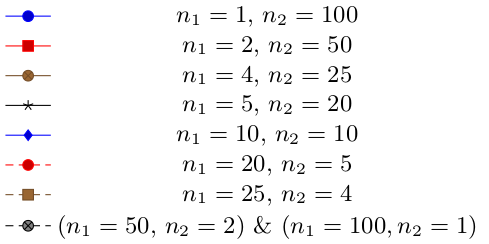
\includegraphics[scale=0.35]{Figs/Legend.png}
\end{subfigure}
\caption{Key Size ratio - Proposed Aggregate Scheme vs Hierarchical Scheme}
\label{plot:keysize}
\end{figure*}

Next, we compare specifically the key size required for the proposed extended scheme, for different values of $n_1$ and $n_2$ (again corresponding to $n=100$), with that required for a hierarchical encryption construction \cite{sandhu1988cryptographic}. Since our scheme uses a hierarchy depth of $2$, we use the same for the hierarchical construction as well, with $n_1$ nodes in level $0$, and $n_2$ level $1$ nodes in the subtree rooted at each level $0$ node. Figure \ref{plot:keysize} summarizes the findings. Evidently, lower the value of $n_1$, better the key aggregation, hence lower the ratio.

\subsection{Utilization Coefficient Comparison}
\label{subsec:util}

Finally we compare the utilization-coefficient of the extended scheme for various values of $n_1$ and $n_2$ (corresponding to $n=100$) with increase in the number of registered key pairs $l$, where each key pair increases the number of classes by $n_2$. We leave out the configuration $n_1=n,n_2=1$ because that always leads to an utilization coefficient of $1$ but is impractical due to huge space requirements. Figure \ref{fig:util} demonstrates that that beyond a certain value of $l$, the combination $(1,n)$ proposed in \cite{chu2014key} has a lower utilization coefficient that all other combinations of $(n_1,n_2)$ for a given $n$. This emphasizes the advantage of making the choice of $(n_1,n_2)$ flexible.

\begin{figure*}[!t]
\captionsetup{font=scriptsize}
\centering
\begin{subfigure}{0.5\textwidth}
\captionsetup{font=scriptsize}
\centering
% \hspace{100.13cm}
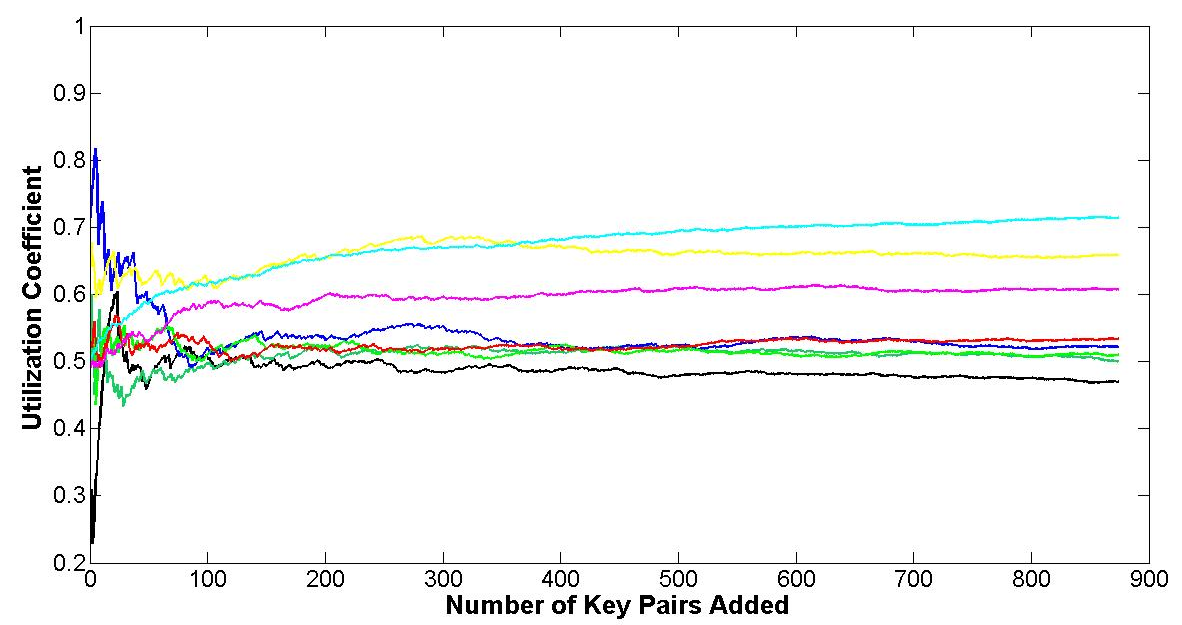
\includegraphics[scale=0.22]{Figs/UtilizationPlot.png}
\end{subfigure}%
\begin{subfigure}{0.5\textwidth}
\captionsetup{font=scriptsize}
\centering
\hspace*{3.13 cm}
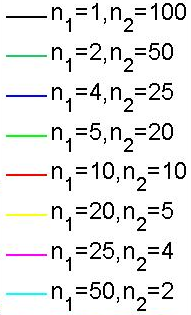
\includegraphics[scale=0.3]{Figs/Legend1.png}
\end{subfigure}
\caption{Utilization coefficient vs Newly Registered Keys}
\label{fig:util}
\end{figure*}


\section{Applications of KAC}
\label{sec:applications}

The key-aggregate encryption systems described in this paper are primarily meant for data sharing on the cloud. In this section, we point out some specific applications in which KAC proves to be a very efficient solution.

\subsection*{Online Collaborative Data Sharing} The foremost application of KAC is in secure data sharing for collaborative applications. Applications such as Google Drive \cite{googledrive} and Dropbox \cite{dropbox} allow users to share their data on the cloud and delegate access rights to multiple users to specific subsets of their whole data. Even government and corporate organizations require secure data sharing mechanisms for their daily operations. KAC can be easily set up to function on top of standard data sharing applications to provide security and flexibility. Data classes may be viewed as folders containing similar files. The fact that our proposed KAC is identity based means that each folder can have its own unique ID chosen by the data owner. Also, the fact that the ciphertext overhead is only logarithmic in the number of data classes implies that space requirement for any data owner is optimal. Finally, the aggregate key also has low overhead and can be transmitted via a secure channel such as a password protected mail service. Since KAC is easily extensible to multiple data owners, the system is practically deployable for a practical data sharing environment. The other advantage of KAC is that once a system is setup with a set of multilinear maps and public parameters, the same setup with the same set of public parameters can be reused by multiple teams within the same organization. Since data owned by each individual owner is insulated from access by users who do not have the corresponding aggregate key, and each data owner has her own tuple of public, private and authentication keys, a single KAC can support multiple data sharing units, while guaranteeing the same underlying security. This saves the cost of setting up new multilinear maps and public parameters each time. 

\subsection*{Distribution of Product License and/or Activation Keys} Suppose a company owns a number of products, and intends to distribute the license files (or activation keys) corresponding to these to different users. The KAC framework allows them to put these keys on the cloud in an encrypted fashion, and distribute an aggregate key corresponding to the license files for multiple products to legally authenticated customers as per their requirements. The legal authentication comes from the fact the user who buys multiple products from the company is given the authentication key and the aggregate key that allows her to decrypt the license file for each product. Since both these keys are of constant size, distributing  these to users is easier than providing a separate license file to each user.

\subsection*{Patient controlled encryption (PCE)} Patient controlled encryption~(PCE) is a recent concept that has been studied in the literature \cite{benaloh2009patient}. PCE allows a patient to upload her own medical data on the cloud and delegate decryption rights to healthcare personnel as per her requirement. KAC acts as an efficient solution to this problem by allowing patients to define their own hierarchy of medical data and delegate decryption rights to this data to different specialists/medical institutions using aggregate keys in an efficient fashion. Given the multitude of sensitive digital health records existent in today's world, storing this data in local/personal machines is not a viable solution and the cloud seems the best alternative. KAC thus provides a two-way advantage in this regard. Not only does it allow people from across the globe to store their health data efficiently and safely, but also allows them to envisage the support of expert medical care from across the globe. 



\section{A Generalized Basic KAC Construction}
\label{sec:general}

In this section, we present a a generalized basic KAC construction. The essential idea is to run $n_A$ parallel instances of the basic scheme parameterized by $n_B$ number of classes, so that the overall system can handle as many as $n=n_A\times n_B$ data classes. Each of these instances share the same set of public parameters, but use their own set of private and public keys. This leads to a trade-off between the overhead for various system parameters. 

\subsection{The Construction}
\label{subsec:two-tier}

We present the construction for generalized KAC in this section. The construction uses techniques similar to the generalized broadcast encryption scheme proposed in \cite{boneh2005collusion}. The generalization in \cite{boneh2005collusion} trades off the ciphertext size with the public key size. Our scheme, on the other hand, trades off the public parameter size with the public key size and the aggregate key size, while still maintaining constant ciphertext overhead.\\

\noindent \textbf{SetUp}$(1^{\lambda},n_B)$: Randomly pick $\alpha \in \mathbb{Z}_q$. Output the system parameter as $param = (P,Q,Y_{P,\alpha,n_B},Y_{Q,\alpha,n_B}))$. Discard $\alpha$. \\

\noindent \textbf{KeyGen}($n_A$): Randomly pick $\gamma_{1},\cdots,\gamma_{n_A} \in \mathbb{Z}_q$. Let $msk_j=\gamma_j$, $PK^1_j=\gamma_{j}P$ and $PK^2_j=\gamma_{j}Q$ for $1\leq j \leq n_A$. Set the master secret key $msk=(msk_1,\cdots,msk_{n_A})$. Set $PK^1=(PK^1_1,\cdots,PK^1_{n_A})$ and $PK^2=(PK^2_1,\cdots,PK^2_{n_A})$. Finally, set the public key $PK=(PK^1,PK^2)$ and output the tuple $(msk,PK)$.\\

\noindent \textbf{Encrypt}$(PK,i,\mathcal{M})$: Compute $a_i=\lceil i/n_B\rceil$ and $b_i=i \text{ mod } B$. Randomly choose $t\in\mathbb{Z}_q$ and output the ciphertext $\mathcal{C}$ as 
 \begin{equation}
 \mathcal{C}=(c_1,c_2,c_3)=(tQ,t(PK^{2}_{a}+Q_{b}),\mathcal{M}.{e}(P_n,tQ_1)) \nonumber
 \end{equation} 

\noindent \textbf{Extract}$(msk,\mathcal{S})$: For the subset of class indices $\mathcal{S}$ and $1\leq a \leq n_A$, define
\begin{eqnarray}
 \mathcal{S}_{a}&=&\{i|i\in\mathcal{S},\lceil i/n_B\rceil=a\} \nonumber\\
 \mathcal{S}'_a&=&\{b_i=i\text{ mod }n_B|i\in\mathcal{S}_{a}\}\nonumber
\end{eqnarray}
\noindent Next, for $1\leq a \leq n_A$, compute
\begin{equation}
 K^{a}_{\mathcal{S}} = {msk_{a}}\sum_{b\in\mathcal{S}'_a}P_{n+1-b} \nonumber
\end{equation}
\noindent Note that this is indirectly equivalent to setting $K^{a}_{\mathcal{S}}$ to $\sum_{b\in\mathcal{S}'_a}\alpha^{n+1-b}PK^{1}_a$. Finally, output 
\begin{equation}
 K_{\mathcal{S}} = (K^{1}_{\mathcal{S}},\cdots,K^{n_A}_{\mathcal{S}})\nonumber
\end{equation}
\noindent Note that the the aggregate key now consists of $n_A$ elements.\\

\noindent \textbf{Decrypt}$(\mathcal{C},i,K_{\mathcal{S}},\mathcal{S})$: If $i\notin\mathcal{S}$, output $\bot$. Otherwise, compute $a_i=\lceil i/n_B\rceil$ and $b_i=i \text{ mod } B$ and set: 
 \begin{eqnarray} 
 A_{\mathcal{S}}&=&\sum_{(b\in\mathcal{S}'_{a_i},b\neq b_i}P_{n+1-b_i+b} \nonumber \\
 B_{\mathcal{S}}&=&\sum_{(b\in\mathcal{S}'_{a_i}}P_{n+1-b} \nonumber  
 \end{eqnarray} 
 \noindent Return the decrypted message $\hat{\mathcal{M}}$ as:
 \begin{equation}
  \hat{\mathcal{M}}=c_3.\frac{{e}(K^{a_i}_{\mathcal{S}}+A_{\mathcal{S}},c_1)}{{e}(B_{\mathcal{S}},c_2)}\nonumber
 \end{equation} 
\noindent Correctness of the algorithm may be easily proved similarly as in Section \ref{subsec:construction1}. Finally, we note that setting $n_A=1$ and $n_B=n$ gives the basic construction of Section \ref{subsec:construction1}. 


\subsection{Performance and Efficiency}
\label{subsec:perf_twotier}

The choice of $n_A$ and $n_B$ play an important role in system performance. As is clear from the construction, the ciphertext always consists of a constant number of group elements. The public parameter comprises of $n_B$ group elements, while the aggregate key as well as the public key consist of $n_A$ group elements each. Thus choosing a smaller value of $n_B$ is useful for applications requiring low overhead aggregate keys. However, choosing $n_A=n_B=\sqrt{n}$ minimizes overall system overhead combining all parameters.

\textbf{We present the simulation studies with different values of $n_A$ and $n_B$ here}.

% We look at the performance of the general KAC construction from the perspective of both parties involved - the data owner sharing her data and an user accessing the shared data. From the data owner's perspective, each superclass comprises of a basic KAC module parameterized with $n$, with constant size public, private and authentication keys. The encryption process can be speeded up using similar caching techniques described in Section \ref{subsec:perf_basic}. From the user's perspective, the system is an ensemble of basic KAC units - one per superclass. For a user willing to access data from $k$ data owners, the aggregate key and authentication keys have size linear in $k$. It seems difficult to do better than this while maintaining data isolation and privacy for each data owner. As in encryption, the decryption process can also be expedited using appropriate caching techniques. It is important to note that the public $param$, which essentially forms the fundamental basic for the security of the general KAC, is a function of $n$ only, and does not depend on the number of users $M$ registered in the system.
% 
% An important aspect of this construction is to decide on an appropriate value for $n$. Keeping a small $n$ value reduces the size of the public parameter. But then a data owner with a large number of data classes $N$ would have to register with $\lceil N/n \rceil$ public, private and authentication key sets, which may not be desirable. Thus there exists a trade-off in using smaller and larger values of $n$ in this scheme. 

% It is important to note that the security of the system depends on the $(n,n)$-BDHE assumption, as we show next.

% \begin{figure*}
% \centering
% \captionsetup{font=scriptsize}
% 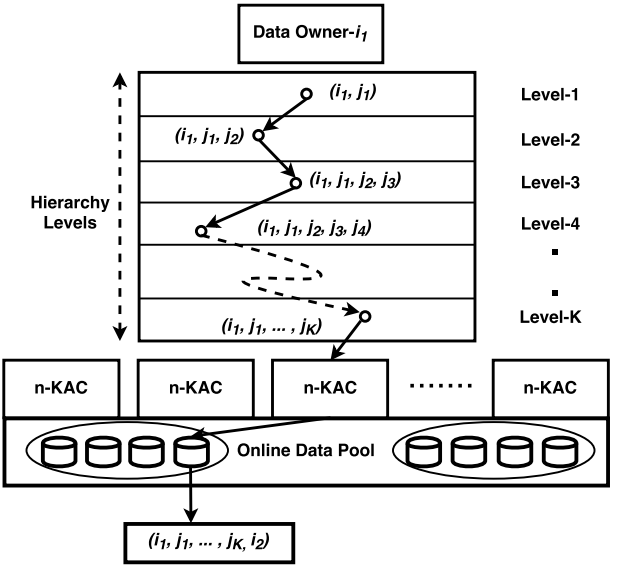
\includegraphics[scale=0.4]{Figs/Hierarchical.png}
% \caption{Hierarchical KAC}
% \label{fig:K-tier}
% \end{figure*}

\subsection{Semantic Security of General KAC}
\label{subsec:security_twotier}

For the non-adaptive CPA security of the generalized KAC construction, we state the following theorem.

\begin{Theorem}
\label{th:twotierCPA}
Let $\mathbb{G}_1$ and $\mathbb{G}_2$ be bilinear elliptic curve subgroups of prime order $q$. For any pair of positive integers $n',n (n'>n)$, the generalized KAC is $(\tau,\epsilon,n')$ CPA secure if the asymmetric decision $(\tau,\epsilon,n)$-BDHE assumption holds in $(\mathbb{G}_1,\mathbb{G}_2)$.
\end{Theorem}

\noindent The proof of this theorem is very similar to the proof of Theorem \ref{th:basicCPA} and is hence avoided.

% \noindent{\textit{Proof:}} Let $\mathcal{A}$ be a $\tau$-time adversary such that $|Adv_{\mathcal{A},n'}-\frac{1}{2}| > \epsilon$ for a two-tier KAC system parameterized with a given $n$. We build an algorithm $\mathcal{B}$ that has advantage at least $\epsilon$ in solving the $(n,n)$-BDHE problem in $(\mathbb{G}_1,\mathbb{G}_2)$. Algorithm $\mathcal{B}$ takes as input a random $(n,n)$-BDHE challenge $(I'=(H',P,Q,Y_{P,\alpha,n},Y_{Q,\alpha,n}),Z')$ (where $Z'$ is either ${e}(P_{n+1},H')$ or a random value in $\mathbb{G}_T$), and proceeds as follows.\\
% 
% \noindent \textbf{Init:} $\mathcal{B}$ runs $\mathcal{A}$ and receives the set $\mathcal{S}$ of ciphertext classes that $\mathcal{A}$ wishes to be challenged on. $\mathcal{B}$ then randomly chooses a ciphertext class $(a,b)\in\mathcal{S}$.\\
% 
% \noindent \textbf{SetUp}: As discussed before, $\mathcal{B}$ should generate the public $param$, public key $PK$, the authentication key $U$, and the aggregate key $K_{\overline{\mathcal{S}}}$ and provide them to $\mathcal{A}$. They are generated as follows.
% %  \vspace{-0.6mm}
%  \begin{itemize}
%   \item $param$ is set as $(P,Q,Y_{P,\alpha,n},Y_{Q,\alpha,n})$.
%   \item $msk^{a}$ is set as some $u$ randomly chosen from $\mathbb{Z}_q$.
%   \item Set $PK^{a}=(PK^{a}_1,PK^{a}_2)$, where $PK^{a}_1$ and $PK^{a}_2$ are computed as $uP - P_{b}$ and $uQ-Q_{b}$ respectively.
%   \item $K^{a}_{\overline{\mathcal{S}}}$ is set as $\sum_{(a,j_2)\notin\mathcal{S}}({u}P_{n+1-j_2}-(P_{n+1-j_2+b}))$.   
%   \item Choose a random $t\in \mathbb{Z}_q$, and set $U^{a}=tQ$.
%  \end{itemize}
%  
% \noindent Since $P$, $Q$ $\alpha$, $U^{a}$ and the $u$ values are chosen uniformly at random, \emph{the public parameters and the public key have an identical distribution to that in the actual construction}. Also note that providing $\mathcal{A}$ with the aggregate key or the authentication key is unnecessary since they do not impart any information about an encrypted message in the class $(a,b)$. \\
% 
% \noindent \textbf{Challenge}: As before, to generate the challenge, $\mathcal{B}$ picks at random two messages $m_0$ and $m_1$ from the set of possible plaintext messages belonging to class $(a,b)$. She randomly picks $b\in\{0,1\}$, and sets the challenge as $(\mathcal{C},m_0,m_1)$, where $\mathcal{C}=(H'-U^{a},uH',m_b.Z')$. We claim that when $Z'={e}(P_{n+1},H')$ (i.e. the input to $\mathcal{B}$ is a valid $(n,n)$-BDHE tuple), then $(\mathcal{C},m_0,m_1)$ is a valid challenge to $\mathcal{A}$ as in a real attack. To see this, we write $H'=t'Q$ for some unknown $t'\in\mathbb{Z}_q$. Then we have $H'-U=rQ$ for some unknown $r=t-t'$, and $uH'$ = $t'(uQ)$ = $t'(uQ-{Q_{b}}+Q_{b})$ = $t'(PK^{a}_2+Q_{b})$. Finally, $m_b.Z'=m_b{e}(P_{n+1},t'Q)$. Thus, by definition, $\mathcal{C}$ is a valid encryption of the message $m_b$ in class $(a,b)$ and hence, $(\mathcal{C},m_0,m_1)$ is a valid challenge to $\mathcal{A}$.\\
% 
% \noindent \textbf{Guess}: The adversary $\mathcal{A}$ outputs a guess $b'$ of $b$. If $b' = b$, $\mathcal{B}$ outputs $0$ (indicating that $Z' = {e}(P_{n+1},H')$). Otherwise, it outputs $1$ (indicating that $Z'$ is a random element in $\mathbb{Z}_T$).\\
%  
% A similar analysis as in Section \ref{subsec:proof_basic} establishes that $\mathcal{B}$ has advantage at least $\epsilon$ in solving the $(n,n)$-BDHE problem in $(\mathbb{G}_1,\mathbb{G}_2)$. This concludes the proof of Theorem \ref{th:twotierCPA}.
% 
% It is important to note that in a practical environment, any data sharing scheme is expected to support a hierarchical organization of data, where different users are given access to different levels of the data. For example, consider an online data pool on the cloud storing an organization's data. The organization (which owns the data) would like to delegate access rights to this data among its employees. Different employees may be given access to different levels of this data depending on their respective credentials and designation. The most common solution to this is to have a pre-defined hierarchical framework for organizing the data, and have keys at different levels of the hierarchy. As pointed out in our previous discussion, highly irregular data access patterns from multiple users could compromise the efficiency of such a hierarchical system by potentially blowing up the size of the key to be shared. Since key aggregation allows us to combine the decryption rights to multiple data classes into a single constant-sized entity, it seems KAC could be the most efficient solution even in this scenario. However, we show next via a small example that the generalized KAC in its original form may not be able to tackle this problem in the most efficient manner.   
% 
% Although the generalized KAC is highly scalable and efficient, it has a drawback in the sense that it fails to support hierarchical organization of data within a single data owner system. Consider the scenario in which a data owner would like to have two distinct folders, namely $F_1$ and $F_2$, that are meant to be accessed by separate user groups. In the generalized KAC framework, she must then have different public, private and authentication keys for these folders. Now if she were to delegate decryption rights to some user for a subset of files both these folders, she would need to provide two aggregate keys, one for each folder. This is because the generalized KAC does not allow her to aggregate these two keys into a single key. If she wants to provide a single aggregate key for both the folders, she would need to have another aggregate system in place to combine these two individual keys. This process is cumbersome and becomes difficult to maintain as the number of hierarchy levels grow. The same disadvantage also persists with the KAC proposed in \cite{chu2014key}. However, since data hierarchy is extremely common in file-based storage systems, we must adopt KAC so as to be able to provide the advantage of key aggregation for any arbitrarily complex hierarchical structure, without the data owner having to worry about the internal details of the aggregation. The modified KAC infrastructure must now support key aggregation at various levels of the hierarchy, while using the same security guarantees provided the fundamental single data owner KAC. This motivates the introduction of an augmented version of the general KAC in the next section, which we refer to as the \emph{hierarchical} KAC.   




% In this section, we focus on building an efficiently extensible version of our proposed scheme that allows an user to economically increase the number of ciphertext classes while registering a new public key-private key pair. We adopt the idea presented in \cite{boneh2005collusion} to develop a hierarchical structure that has multiple instances (say $M$) of the original scheme running in parallel. Each such instance in turn provides \emph{locally aggregate keys} for $n$ ciphertext sub-classes. Each ciphertext class thus now has a double index $(a,b)$ where $1\leq a \leq M$ and $1\leq b \leq n$. This allows the overall setup to handle $n=Mn$ classes. However, it is important to note that all the instances can use the same public parameters. This interaction among the instances helps to largely improve performance. We further point out that while in \cite{boneh2005collusion}, the two-tier construction offers a trade-off between the public parameter size and the ciphertext size, our 
% two-tier scheme actually reduces the public parameter size without compromising on the size of the ciphertext. Further, addition of a single new key increases the number of classes only by $n$ and not by $n$. Setting $n\ll n$ thus achieves significant improvement in performance over the existing proposal.


% \subsection{The Construction of the Two-tier KAC}
% \label{subsec:construction2}
% 
% Let $n$ be a fixed positive integer. Our proposed $n$-two-tier key-aggregate encryption scheme over elliptic curve subgroups is as described below. It may be noted that the bilinear additive elliptic curve sub-group $\mathbb{G}$ and the multiplicative group $\mathbb{G}_T$, as well as the pairing $\hat{e'}$ are the same as in the basic scheme. The algorithm sets up $M=\lfloor n/n\rfloor$ instances of the basic scheme, each of which handles $n$ ciphertext classes. The original scheme is thus a special case of the extended scheme with $M=1$ and $n=n$.
% 
% 
% \begin{enumerate}
%  \item \textbf{Setup}$(1^{\lambda},n)$: Randomly pick $\alpha \in \mathbb{Z}_q$. Compute $P_i$ = ${\alpha^{i}}P \in \mathbb{G}$ for $i = 1,\cdots,n,n+2,\cdots,2n$. Output the system parameter as $param$ = $(P,P_1,\cdots,P_{n},P_{n+2},\cdots,P_{2n})$. The system randomly chooses a secret parameter $t \in \mathbb{Z}_q$ which is not made public. It is only known to data owners with credentials to control client access rights.
%  \item \textbf{Keygen}(): Pick $\gamma_1,\gamma_2,\cdots,\gamma_{M} \in \mathbb{Z}_q$, output the public and master-secret key pair: $PK$=$({pk}_1,pk_{2},\cdots,pk_{M})$=$(\gamma_1P,\gamma_2P,\cdots,\gamma_{M}P)$, and $msk$=$(\gamma_1,\gamma_2,\cdots,\gamma_{M})$.
%  \item \textbf{Encrypt}$(pk_{a},(a,b),m)$: For a message $m \in \mathbb{G}_T$ and an index $(a,b) \in \{1,2,\cdots,M\}\times\{1,2,\cdots,n\}$, randomly choose $r\in\mathbb{Z}_q$ and let $t'=t+r \in\mathbb{Z}_q$. Then compute the ciphertext $\mathcal{C}$=$(rP,t'{(pk_{a}+P_{b})},m.\hat{e'}(P_{n},t'P_1))$ = $(c_1,c_2,c_3)$.
%  \item \textbf{Extract}$(msk=\gamma,\mathcal{S})$: For the set $\mathcal{S}$ of indices $(\hat{a},j_2)$ the aggregate key is computed as $K_{\mathcal{S}}$ = $(k^{1}_{\mathcal{S}},k^{2}_{\mathcal{S}},\cdots,k^{M}_{\mathcal{S}})$, where $k^{i}_{\mathcal{S}}$ = $\sum_{(i,j_2)\in\mathcal{S}}{\gamma_{1}}P_{n+1-j_2}$. The dynamic access control parameter $U$ is computed as $tP$. Thus the net aggregate key is $(K_{\mathcal{S}},U)$ which is transmitted via a secure channel to users that have access rights to $\mathbb{S}$. Note that  $k^{\hat{a}}_{\mathcal{S}}=\sum_{(\hat{a},j_2)\in\mathcal{S}}\alpha^{n+1-j}pk_{\hat{a}}$ for $\hat{a}=1,2,\cdots,M$. 
%  \item \textbf{Decrypt}$(K_{\mathcal{S}}, U, \mathcal{S},(a,b),\mathcal{C}=\{c_1,c_2,c_3\})$: If $(a,b)\notin\mathcal{S}$, output $\bot$. Otherwise return the message $\hat{m}$ = $c_3\frac{\hat{e'}(k^{a}_{\mathcal{S}}+\sum_{(a,j_2)\in\mathcal{S},j_2\neq b}P_{n+1-j_2+b},U+c_1)}{\hat{e'}(\sum_{(a,j_2)\in\mathcal{S}}P_{n+1-j_2},c_2)}$. 
% \end{enumerate}
% 
% The proof of correctness for the two-tier scheme is presented below.
% 
% \begin{scriptsize}
% \begin{equation}
% \begin{split}
%  \hat{m} &= c_3\frac{\hat{e'}(k^{a}_{\mathcal{S}}+\sum_{(a,j_2)\in\mathcal{S},j_2\neq b}P_{n+1-j_2+b},U+c_1)}{\hat{e'}(\sum_{(a,j_2)\in\mathcal{S}}P_{n+1-j_2},c_2)}\\
%   &= c_3\frac{\hat{e'}(\sum_{(a,j_2)\in \mathcal{S}}{\gamma_{a}}P_{n+1-j_2} + \sum_{(a,j_2)\in\mathcal{S},j_2\neq b}P_{n+1-j_2+b},t'P)}{\hat{e'}(\sum_{(a,j_2)\in\mathcal{S}}P_{n+1-j_2},t'(pk_{a}+P_{b})}\\
% %   &= c_3\frac{\hat{e'}(\sum_{(a,j_2)\in \mathcal{S}}{\gamma_{a}}P_{n+1-j_2},t'P)\hat{e'}(\sum_{(a,j_2)\in\mathcal{S}}(P_{n+1-j_2+b})-P_{n+1},t'P)}{\hat{e'}(\sum_{(a,j_2)\in\mathcal{S}}P_{n+1-j_2},t'pk_{a})\hat{e'}(\sum_{(a,j_2)\in\mathcal{S}}P_{n+1-j_2},t'P_{b})}\\
%   &= c_3\frac{\hat{e'}(\sum_{(a,j_2)\in\mathcal{S}}P_{n+1-j_2+b},t'P)}{\hat{e'}(P_{n+1},t'P)\hat{e'}(\sum_{(a,j_2)\in\mathcal{S}}P_{n+1-j_2},t'P_{b})}\\
%   &= c_3\frac{\hat{e'}(\sum_{(a,j_2)\in\mathcal{S}}P_{n+1-j_2+b},t'P)}{\hat{e'}(P_{n+1},t'P)\hat{e'}(\sum_{(a,j_2)\in\mathcal{S}}P_{n+1-j_2+b},t'P)}\\
%   &= m\frac{\hat{e'}(P_{n},t'P_1)}{\hat{e'}(P_{n+1},t'P)}\\
%   &= m
% \end{split}  
% \end{equation}
% \end{scriptsize}
% 
% 
% \subsection{Semantic Security of the Two-tier KAC}
% \label{subsec:proof_general}
% 
% \subsubsection{The Reduced Two-tier Scheme:}
% 
% We define a reduced version of the two-tier encryption scheme. We note that the ciphertext $\mathcal{C}=(c_1,c_2,c_3)$ output by the $Encypt$ operation essentially embeds the value of $m$ in $c_3$ by multiplying it with $\hat{e'}(P_{n},tP_1)$. Consequently, the security of our proposed scheme is equivalent to that of a \emph{reduced} two-tier key-aggregate encryption scheme that simply uses the reduced ciphertext $(c_1,c_2)$, the aggregate key $K_{\mathcal{S}}$ and the dynamic access parameter $U$ to successfully transmit and decrypt the value of $\hat{e'}(P_{n},t'P_1)=\hat{e'}(P_{n+1},t'P)$. We prove the semantic security of this \emph{reduced scheme} parameterized with a given number of ciphertext classes $n$ for each instance, which also amounts to proving the semantic security of our original encryption scheme for the same number of ciphertext classes. Note that the proof of security is independent of the number of instances $M$ that run in parallel.
% 
% \subsubsection{The Adversarial Model:} We make the following assumptions about the adversary $\mathcal{A}$:
% 
% \begin{enumerate}
%  \item The adversary has the aggregate key that allows her to access any ciphertext class other than those in the target subset $\mathcal{S}$, that is, she possesses $K_{\overline{\mathcal{S}}}$.
%  \item The adversary has access to the public parameters $param$ and $PK$, and also possesses the dynamic access parameter $U$.
% %  \item The adversary is authorized and and hence 
% \end{enumerate}
% 
% 
% \subsubsection{The Security Proof:}
% 
% The security proof presented here uses the first complexity assumption stated in \ref{subsubsec:asm_1}. Let $\mathbb{G}$ be a bilinear elliptic curve subgroup of prime order $q$. For any pair of positive integers $n,n' (n'>n)$ our proposed $n$-two-tier reduced key-aggregate encryption scheme over elliptic curve subgroups is $(\tau,\epsilon,n')$ semantically secure if the decision $(\tau,\epsilon,n)$-BDHE assumption holds in $\mathbb{G}$. We now prove this statement below.
% 
% \textbf{\noindent{Proof:}} Let for a given input $n'$, $\mathcal{A}$ be a $\tau$-time adversary that has advantage greater than $\epsilon$ for the \emph{reduced scheme} parameterized with a given $n$. We build an algorithm $\mathcal{B}$ that has advantage at least $\epsilon$ in solving the $n$-BDHE problem in $\mathbb{G}$. Algorithm $\mathcal{B}$ takes as input a random $n$-BDHE challenge $(P,H,Y_{(P,\alpha,n)},Z)$ where $Z$ is either $\hat{e'}(P_{n+1},H)$ or a random value in $\mathbb{G}_T$. Algorithm $\mathcal{B}$ proceeds as follows.
% 
% \begin{enumerate}
%  \item \textbf{Init:} Algorithm $\mathcal{B}$ runs $\mathcal{A}$ and receives the set $\mathcal{S}$ of ciphertext classes that $\mathcal{A}$ wishes to be challenged on. For each ciphertext class $(a,b)\in\mathcal{S}$, $\mathcal{B}$ performs the \textbf{SetUp}-$\mathbf{(a,b)}$, \textbf{Challenge}-$\mathbf{(a,b)}$ and \textbf{Guess}-$\mathbf{(a,b)}$ steps. Note that the number of iterations is polynomial in $|S|$. 
%  
%  \item \textbf{SetUp}-$\mathbf{(a,b)}$: $\mathcal{B}$ should generate the public $param$, public key $PK$, the access parameter $U$, and the aggregate key $K_{\overline{\mathcal{S}}}$. For the iteration corresponding to ciphertext class $(a,b)$, they are generated as follows.
%  \begin{itemize}
%   \item $param$ is set as $(P,Y_{P,\alpha,n})$.
%   \item Randomly generate $u_1,u_2,\cdots,u_{M} \in \mathbb{Z}_q$. Then, set $PK$= $(pk_1,pk_2,\cdots,pk_{M})$, with $pk_{\hat{a}}$ = $u_{\hat{a}}P - P_{b}$ for $\hat{a}=1,2,\cdots,M$.
%   \item Set $K_{\overline{\mathcal{S}}}$ = $(k^{1}_{\overline{\mathcal{S}}},k^{2}_{\overline{\mathcal{S}}},\cdots,k^{M}_{\overline{\mathcal{S}}})$, where $k^{\hat{a}}_{\overline{\mathcal{S}}}$ is set as $\sum_{(\hat{a},j_2)\notin\mathcal{S}}({u_{\hat{a}}}P_{n+1-j_2}-(P_{n+1-j_2+b}))$. Then, $k^{\hat{a}}_{\overline{\mathcal{S}}}$ = $\sum_{(\hat{a},j_2)\notin\mathcal{S}}\alpha^{n+1-j_2}pk_{\hat{a}}$,which is as per the scheme specification. Note that $\mathcal{B}$ knows that $(a,b)\notin \overline{\mathcal{S}}$, and hence has all the resources to compute this aggregate key for $\overline{\mathcal{S}}$. 
%   \item $U$ is set as some random element in $\mathbb{G}$.
%  \end{itemize}
%  
%  Note that since $P$, $\alpha$, $U$ and the $u_{\hat{a}}$ values are chosen uniformly at random, the public key has an identical distribution to that in the actual construction.
%  
%  \item \textbf{Challenge}-$\mathbf{(a,b)}$: To generate the challenge for the ciphertext class $(a,b)$, $\mathcal{B}$ computes $(c_1,c_2)$ as $(H-U,u_{a}H)$. It then randomly chooses a bit $b\in{(0,1)}$ and sets $K_b$ as $Z$ and $K_{1-b}$ as a random element in $\mathbb{G}_T$. The challenge given to $\mathcal{A}$ is $((c_1,c_2),K_0,K_1)$. 
%  
%  We claim that when $Z=\hat{e'}(P_{n+1},H)$ (i.e. the input to $\mathcal{B}$ is a $n$-BDHE tuple), then $((c_1,c_2),K_0,K_1)$ is a valid challenge to $A$. We prove this claim here. we point out that $P$ is a generator of $\mathbb{G}$ and so $H=t'P$ for some $t'\in\mathbb{Z}_q$. Putting $H$ as $t'P$ gives us the following:
%  \begin{itemize}
%   \item  $U=tP$ for some $t\in\mathbb{Z}_q$
%   \item $c_1=H-U=(t'-t)P=rP$ for $r=t'-t$
%   \item $c_2=u_{a}H=(u_{a})t'P=t'(u_{a}P)=t'(u_{a}P-P_{b}+P_{b})=t'(pk_{a}+P_{b})$
%   \item $K_b=Z=\hat{e'}(P_{n+1},H)=\hat{e'}(P_{n+1},t'P)$
%  \end{itemize}
%  On the other hand, if $Z$ is a random element in $\mathbb{G}_T$ (i.e. the input to $\mathcal{B}$ is a random tuple), then $K_0$ and $K_1$ are just random independent elements of $\mathbb{G}_T$.
%  
%  \item\textbf{Guess}-$\mathbf{(a,b)}$: The adversary $\mathcal{A}$ outputs a guess $b'$ of $b$. If $b' = b$, $\mathcal{B}$ outputs $0$ (indicating that $Z = \hat{e'}(P_{n+1},H)$), and terminates. Otherwise, it goes for the next ciphertext class in $\mathcal{S}$.
% \end{enumerate}
% If after $|\mathcal{S}|$ iterations, $b' \neq b$ for each ciphertext class $(a,b)\in\mathcal{S}$, the algorithm $\mathcal{B}$ outputs $1$ (indicating that $Z$ is random in $\mathbb{G}_T$). We now analyze the probability that $\mathcal{B}$ gives a correct output. If $(P,H,Y_{(P,\alpha,n)},Z)$ is sampled from $R$-BDHE, $Pr[\mathcal{B}(G,H,Y_{(P,\alpha,n)},Z)=0]$ = $\frac{1}{2}$, while if $(P,H,Y_{(P,\alpha,n)},Z)$ is sampled from $L$-BDHE, $|Pr[\mathcal{B}(G,H,Y_{(P,\alpha,n)},Z)]-\frac{1}{2}|$ $\geq$ $\epsilon$. So, the probability that $\mathcal{B}$ outputs correctly is at least $1-(\frac{1}{2}-\epsilon)^{|\mathcal{S}|} \geq \frac{1}{2}+\epsilon$. Thus $\mathcal{B}$ has advantage at least $\epsilon$ in solving the $n$-BDHE problem. This concludes the proof. \emph{Note that the instance of this proof with $M=1$ and $n=n$ serves as the proof of security for the basic KAC scheme proposed in Section \ref{sec:proposal}}.
% 
% 
% \subsubsection{Performance Trade off with the Basic Scheme:} 
% 
% We compare the various parameter sizes for the proposed original and extended schemes in table \ref{tab:tradeoff}. We note that $SetUp$ and $KeyGen$ are both one-time operations, and for a given subset $\mathcal{S}$, the $Extract$ operation is also performed once to generate the corresponding aggregate key $K_{\mathcal{S}}$. The most important advantage that the two-tier scheme provides is the user's ability to efficiently extend the number of ciphertext classes. As far as encryption and decryption are concerned, encryption should ideally take the same time for both schemes, while decryption is actually expected to be faster for the two-tier construction as $n\leq n$.  
% 
% \begin{table}[!t]
% \captionsetup{font=scriptsize}
% \caption{Comparison between the Basic and Two-tier schemes}
% \label{tab:tradeoff}
% \begin{center}
% \scalebox{0.75}{
% \begin{tabular}{|c|c|c|c|}
% 
% %Symbol & Fault Model \\
% %(MHz)&$\ $ &$\ $ & $\ $\\
% \hline
% \textbf{Item} & \textbf{Nature of Computation} & \textbf{Original scheme} & \textbf{Two-tier scheme}\\\hline\hline
% 
% $param$(SetUp) & One-time & $\mathcal{O}(n)$ & $\mathcal{O}(n)$\\\hline
% $PK$(KeyGen) & One-time &$\mathcal{O}(1)$ & $\mathcal{O}(M)$\\\hline
% $K_{\mathcal{S}}$(Extract) & One-time & $\mathcal{O}(1)$ & $\mathcal{O}(M)$\\\hline
% $\mathcal{C}$ & One per Message & $\mathcal{O}(1)$ & $\mathcal{O}(1)$\\\hline
% Encrypt & One Per Message & $\mathcal{O}(1)$ & $\mathcal{O}(1)$\\\hline
% Decrypt & One Per Message & $\mathcal{O}(|\mathcal{S}|)$ & $\mathcal{O}(|\mathcal{S}|)$\\\hline
% % Ciphertext Class Extension & Dynamic & Not Possible & $\mathcal{O}(n)$\\\hline
% \hline
% % OSB & Other Single Byte Faults (More than 4 bits in one byte affected)  \\
% % MB & Multiple Byte Faults  \\
% 
% % \hline \hline
% \end{tabular}
% }
% 
% \end{center}
% \end{table}
% 
% 
% \subsection{A Flexible Extension Policy}
% \label{subsec:extension}
% 
% If a user needs to classify her ciphertexts into more that $n$ classes, she can register for additional key pairs $(pk_{M+1},msk_{M+1})$, $\cdots$, $(pk_{M+l},msk_{M+l})$ as per her requirements. Each new key registration increases the number of classes by $n$, where $n\leq n$. The idea of under-utilization stems from the fact that registration of each public-private key pair increases the number of classes by $n$. However, it is not necessary that all the existing classes are utilized at any given point of time. For instance, a user may at any point of time want to register $l$ new private-public key pairs, however she will in all probability not use up all $ln$ additional classes of messages that could be encrypted using the newly registered keys. We stress here is that, unlike in the public key extension scheme proposed in \cite{chu2014key} where the values of $M$ and $n$ are fixed to $1$ and $n$ respectively, our two-tier construction \emph{provides a choice} of $M$ and $n$ so that the system administrator could choose pair of values suited to their requirements. 
% 
% We propose a metric to quantify the under-utilization of ciphertext classes for a given configuration of the system. Let us assume that at some instance of time, there are $M+l$ private-public key pairs registered in the system, and $c_i$ classes corresponding to each key are being utilized. We define the utilization coefficient as $\frac{1}{1+\xi}$, where $\xi=-\frac{1}{M}\sum_{i=1\\c_i\neq0}^{M}\log(\frac{c_i}{n})$. An efficient scheme tries to minimize the value of $\xi$ to achieve good utilization of the existing set of classes. The value is maximum when $c_i=n \forall i=1,2,\cdots,n$. Note that $c_i=0$ implies that no subclasses under the given key $pk_i$ are being utilized, which is equivalent to not registering the key at all.        
% 
% 
% To stress the importance of the flexible extension policy, we provide a simplified example here. We consider two possible configurations of the extended scheme. In the first configuration, $M=1$ and $n=n$, which is essentially identical to the public key extension scheme proposed in \cite{chu2014key}. The other configuration has $M>1$ and $n<n$. Now assume that before extension, both schemes utilized $c$ ciphertext classes out of the $n$ possible classes, equally distributed across all key pairs. Now suppose a situation arises where an user needs to register $l$ more key pairs, and utilizes $z<n$ classes corresponding to each key. In the first configuration, we have $\xa=-\frac{1}{l+1}(l\log(\frac{z}{n})+\log(\frac{c}{n}))$, while for the second configuration, $\xb=-\frac{1}{l+M}(l(\log(\frac{z}{n}))+M\log(\frac{c}{n}))$. Now for $l>(\frac{M}{\log M}-1)\log(\frac{z}{c})-1$, $\xb<\xa$. Thus for any value of $(M,n)$ other than $(1,n)$, there exists a value of $l$ for which the 
% scheme achieves better utilization coefficient. Since $l$ is expected to increase in a dynamic scenario, our public key extension scheme eventually performs better than the scheme suggested in \cite{chu2014key}. 
% 
% \subsection{Advantage over Hierarchical Encryption Based Schemes}
% \label{subsec:advantage}
% 
% \begin{figure}[!t]
% \centering
% \captionsetup{font=scriptsize}
% 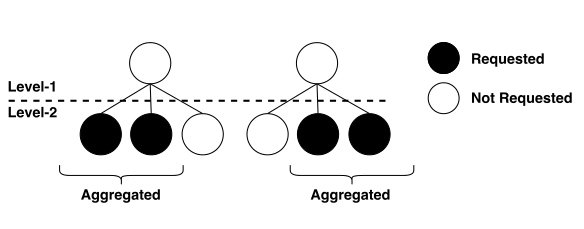
\includegraphics[scale=0.4]{Figs/tree.png}
% \caption{A Practical Request Scenario in the Hierarchical Setting}
% \label{fig:agg}
% \end{figure}
% 
% Although the two-tier scheme has a two level hierarchy (with each of the $M$ parallely executing instances of the basic scheme representing a node in the top level and the actual ciphertext classes representing nodes in the lower level), it avoids the pitfalls of existing hierarchical encryption based schemes \cite{akl1983cryptographic,ateniese2012provably}. In standard tree based hierarchical systems, granting access to the key corresponding to any node implicitly grants access to all the keys in the subtree rooted at that node. This means granting access to a selected set of nodes in a given subtree would blow up the key-size to be the same as the number of nodes. This is avoided in our two-tier scheme, since any number of nodes (ciphertext classes) that belong to the same instance may be aggregated into a single key. Figure \ref{fig:agg} summarizes this phenomenon. In the situation depicted, a tree-based hierarchy system would require $4$ decryption keys, while our 
% scheme would require only $2$. In this respect, our scheme has similar advantages to that of \cite{chu2014key}.
% 
% 
% 
% 
% 
% 
% 
% 
% 
% 
% 

\section{Extending Dynamic KAC for Chosen Ciphertext Security}
\label{sec:CCA}

We now demonstrate how to extend dynamic KAC to obtain chosen ciphertext security. For clarity of understanding, we demonstrate the extension for the basic dynamic KAC proposed in Section \ref{sec:proposal}. The resulting KAC system is CCA secure \emph{without using random oracles}. To the best of our knowledge, this is the first CCA secure KAC proposed in literature. The extension methodology is inspired by ideas presented in \cite{boneh2005collusion}. The extensions for the two-tier and $M$-tier scheme, follow similarly.

\subsection{Additional Requirements}
\label{subsec:additional}

We have the following additional requirements for the CCA secure dynamic KAC:

\begin{itemize}
 \item A signature scheme $(SigKeyGen,Sign,Verify)$. 
 \item A collision resistant hash function for mapping verification keys to $\mathbb{Z}_q$. 
\end{itemize}

For simplicity of presentation, we assume here that the signature verification keys are encoded as elements of $\mathbb{Z}_q$. Hence the hash function is not mentioned in each location, since it is implicit that any signature value we refer to in the forthcoming discussion is essentially the hash value corresponding to the original signature.

\subsection{The Construction of CCA-Secure Dynamic KAC}
\label{subsec:construction_CCA}

We will demonstrate in the following section that the security of CCA-secure Dynamic KAC for $n$ ciphertext classes is based on the $(n+1)$-BDHE assumption, instead of the $n$-BDHE assumption for the basic scheme. For consistency of notation, we describe here the CCA-secure dynamic KAC for $n-1$ users, such that the security assumption is still the $n$-BDHE assumption as before. We now describe the working of the system. Note that the bilinear additive elliptic curve sub-group $\mathbb{G}$ and the multiplicative group $\mathbb{G}_T$, as well as the pairing $\hat{e'}$ are the same as described so far. 

\begin{enumerate}
 \item \textbf{Setup}$(1^{\lambda},n-1)$: Randomly pick $\alpha \in \mathbb{Z}_q$. Compute $P_i = {\alpha^{i}}P \in \mathbb{G}$ for $i = 1,\cdots,n,n+2,\cdots,2n$. Output the system parameter as\\
 $param = (P,P_1,\cdots,P_n,P_{n+2},\cdots,P_{2n})$. The system also randomly chooses a secret parameter $t \in \mathbb{Z}_q$ which is not made public. It is only known to data owners with credentials to control client access rights.
 \item \textbf{Keygen}(): Pick $\gamma \in \mathbb{Z}_q$, output the public and master-secret key pair : \\$(PK={\gamma}P,msk=\gamma)$.
 \item \textbf{Encrypt}$(PK,i,m)$: Run the $SigKeyGen$ algorithm to obtain a signature signing key $K_{SIG}$ and a verification key $V_{SIG} \in \mathbb{Z}_q$. Then, randomly choose $r\in\mathbb{Z}_q$ and let $t'=t+r \in\mathbb{Z}_q$. Then compute\\ $\mathcal{C}'=(rP,t'{(PK+P_i+V_{SIG}P_n)},m.\hat{e'}(P_n,t'P_1),)$ $=$ $(c_1,c_2,c_3)$. Output the ciphertext\\
 $\mathcal{C}=(\mathcal{C}',Sign(\mathcal{C}',K_{SIG}),V_{SIG})$.
 \item \textbf{Extract}$(msk=\gamma,\mathcal{S})$: For the set $\mathcal{S}$ of indices $j$ the aggregate key is computed as\\ $K_{\mathcal{S}} = \sum_{j\in\mathcal{S}}{\gamma}P_{n+1-j}$ = $\sum_{j\in\mathcal{S}}\alpha^{n+1-j}PK$\\ and the dynamic access control parameter $U$ is computed as $tP$. Thus the net aggregate key is $(K_{\mathcal{S}},U)$ which is transmitted via a secure channel to users that have access rights to $\mathbb{S}$.
 \item \textbf{Decrypt}$(K_{\mathcal{S}}, U, \mathcal{S},i,\mathcal{C})$: Let $\mathcal{C}=(\mathcal{C}',\sigma,V_{SIG})$. Verify that $\sigma$ is a valid signature of $\mathcal{C}'$ under the key $V_{SIG}$. If not, output $\bot$. Also, if $i\notin\mathcal{S}$, output $\bot$. Otherwise, pick a random $w\in \mathbb{Z}_q$. Let $SIG_{mathcal{S}}=\sum_{j\in\mathcal{S}}V_{SIG}P_{2n+1-j}$. This can be computed as $1\leq j\leq n-1$. Next, compute\\ $\hat{d_1}=K_{\mathcal{S}}+SIG_{\mathcal{S}}+\sum_{j\in\mathcal{S},j\neq i}P_{n+1-j+i} + w(PK+P_i+V_{SIG}P_n)$, and $\hat{d_2}=(\sum_{j\in\mathcal{S}}P_{n+1-j})+wP$. Return the message $\hat{m}=c_3\frac{\hat{e'}(\hat{d_1},U+c_1)}{\hat{e'}(\hat{d_2},c_2)}$. 
\end{enumerate}

The proof of correctness of this scheme is very similar to the proof for the basic dynamic KAC scheme presented in Section \ref{sec:proposal}, and it can be easily shown that $\frac{\hat{e'}(\hat{d_2},c_2)}{\hat{e'}(\hat{d_1},U+c_1)}=\hat{e'}(P_n,t'P_1)$. Note that the ciphertext size is still constant and everything else, including the public and private parameters, as well as the aggregate key, remains unchanged. The main change from the original scheme is in the fact that decryption requires a randomization value $w\in\mathbb{Z}_q$. This randomization makes sure that that the pair $(\hat{d_1},\hat{d_2})$ is chosen from the distribution $(x(PK+P_i+V_{SIG}P_n)-P_{n+1},xP)$ where $x$ is chosen uniformly from $\mathbb{Z}_q$. To verify this claim, set $x=w+\sum_{j\in\mathcal{S}}\alpha^{n+1-j}$. Then $\hat{d_2}=xP$ and $\hat{d_1}=x(PK+P_i+V_{SIG}P_n)-P_{n+1}$. Also, since $w$ is uniformly random in $\mathbb{Z}_q$, so is $x$. \emph{This randomization is a vital aspect from the point of view of CCA-security}.

 
\subsection{Proof of CCA-Security}
\label{subsec:proof_cca}

We begin by pointing out that a signature scheme $(SigKeyGen,Sign,Verify)$ is $(t,\epsilon,q_S)$ strongly existentially unforgeable if no $t$-time adversary who makes at most $q_{S}$ signature signature queries and is unable to produce some new (message,signature) pair with probability at least $\epsilon$ \cite{}. The proof of security uses a reduced version of the modified KAC scheme, analogous to the reduced scheme used for proving the security of the basic KAC. The adversarial model is also the assumed to be the same as for the basic KAC. Once again, the security proof presented here uses the first complexity assumption stated in \ref{subsubsec:asm_1}. Let $\mathbb{G}$ be a bilinear elliptic curve subgroup of prime order $q$. For any pair of positive integer $n$ the modified reduced key-aggregate encryption scheme is $(\tau,\epsilon_1+\epsilon_2,n-1,q_D)$ CCA-secure if the decision $(\tau,\epsilon_1,n)$-BDHE assumption holds in $\mathbb{G}$ and the signature scheme is $(t,\epsilon_2,1)$ strongly existentially unforgeable.

\textbf{\noindent{Proof:}} Let $\mathcal{A}$ be a $\tau$-time adversary that has advantage greater than $\epsilon_1+\epsilon_2$ in solving the \emph{reduced scheme} parameterized with a fixed $n$. Using $\mathcal{A}$, we build an algorithm $\mathcal{B}$ that has advantage at least $\epsilon_1$ in solving the $n$-BDHE problem in $\mathbb{G}$. Algorithm $\mathcal{B}$ takes as input a random $n$-BDHE challenge $(P,H,Y_{(P,\alpha,n)},Z)$ (where $Z$ is either $\hat{e'}(P_{n+1},H)$ or a random value in $\mathbb{G}_T$), and proceeds as follows.

\begin{enumerate}
 \item \textbf{Init:} $\mathcal{B}$ runs $\mathcal{A}$ and receives the set ${\mathcal{S}}^{*}$ of ciphertext classes that $\mathcal{A}$ wishes to be challenged on. For each ciphertext class $i\in\mathcal{S}$, challenger $\mathcal{B}$ performs the \textbf{SetUp}-$\mathbf{i}$, \textbf{Query Phase 1}-$\mathbf{i}$, \textbf{Challenge}-$\mathbf{i}$, \textbf{Query Phase 2}-$\mathbf{i}$ and \textbf{Guess}-$\mathbf{i}$ steps. Note that the number of iterations is polynomial in ${\mathcal{S}}^{*}$. Note that the number of iterations is polynomial in $|{\mathcal{S}}^{*}|$. 
 
 \item \textbf{SetUp}-$\mathbf{i}$: $\mathcal{B}$ should generate the public $param$, public key $PK$, the access parameter $U$, and the aggregate key $K_{\overline{{\mathcal{S}}^{*}}}$ and provide them to $\mathcal{A}$. Algorithm $\mathcal{B}$ first runs the $SigKeyGen$ algorithm to obtain a signature signing key ${K^{*}}_{SIG}$ and a corresponding verification key ${V^{*}}_{SIG} \in \mathbb{Z}_q$. The various items to be provided to $\mathcal{A}$ are generated as follows.
%  \vspace{-0.6mm}
 \begin{itemize}
  \item $param$ is set as $(P,Y_{P,\alpha,n})$.
  \item $PK$ is set as $uP - {V^{*}}_{SIG}P_n - P_i$ where $u$ is randomly chosen from $\mathbb{Z}_q$.
  \item $K_{\overline{{\mathcal{S}}^{*}}}$ is set as $\sum_{j\notin{\mathcal{S}}^{*}}({u}P_{n+1-j}- {V^{*}}_{SIG}P_{2n+1-j} -P_{n+1-j+i})$. Note that $K_{\overline{{\mathcal{S}}^{*}}}$ is equal to $\sum_{j\notin{\mathcal{S}}^{*}}\alpha^{n+1-j}PK$, in accordance with the specification provided by the scheme. Moreover, $\mathcal{B}$ is aware that $i\notin \overline{{\mathcal{S}}^{*}}$ (implying $i\neq j$). Also, $j\neq n$ as $1\leq j \leq n-1$. Hence, $\mathcal{B}$ has all the resources to compute $K_{\overline{{\mathcal{S}}^{*}}}$.
  \item $U$ is set as some random element in $\mathbb{G}$.
  
 \end{itemize}
 
 Since $P$, $\alpha$, $U$ and the $u$ values are chosen uniformly at random, \emph{the public parameters and the public key have an identical distribution to that in the actual construction}.
 
 \item \textbf{Query Phase 1}-$\mathbf{i}$: Algorithm $\mathcal{A}$ issues decryption queries. Let $(j,\mathcal{S},\mathcal{C})$ be a decryption query where $\mathcal{S}\subseteq{\mathcal{S}}^{*}$ and $j\in\mathcal{S}$. Let $\mathcal{C}=((c_1,c_2),\sigma,V_{SIG})$. Algorithm $\mathcal{B}$ first runs $Verify$ to check if the signature $\sigma$ is valid on $(c_1,c_2)$ using $V_{SIG}$. If invalid, $\mathcal{B}$ returns $\bot$. If $V_{SIG} = {V^{*}}_{SIG}$, $\mathcal{B}$ outputs a random bit $b\in\{0,1\}$ and \emph{aborts} the simulation. Otherwise, the challenger picks a random $x\in\mathbb{Z}_q$. It then sets $\hat{d_2}=xP+{(V_{SIG}-{V^{*}}_{SIG})}^{-1}P_1$, and $\hat{d_1}=u\hat{d_2}+x(V_{SIG}-{V^{*}}_{SIG})P_n$. $\mathcal{B}$ responds with $K=\frac{\hat{e'}(\hat{d_2},c_2)}{\hat{e'}(\hat{d_1},c_1 + U)}$. To see that this response is as in a real attack game, let $x'=x+\alpha{(V_{SIG}-{V^{*}}_{SIG})}^{-1}$. Then $\hat{d_2}=x'P$ and $\hat{d_1}=x'(PK+P_i+V_{SIG}P_n)-P_{n+1}$. Furthermore, since $x$ is uniform in $\mathbb{Z}_q$, $x'$ is also uniform in $\mathbb{Z}_q$. 
 
 \item \textbf{Challenge}-$\mathbf{i}$: To generate the challenge for the ciphertext class $i$, $\mathcal{B}$ computes $(c_1,c_2)$ as $(H-U,uH)$. It sets ${\mathcal{C}}^{*}=((c_1,c_2),Sign((c_1,c_2),{K^{*}}_{SIG}),{V^{*}}_{SIG})$. It then randomly chooses a bit $b\in{(0,1)}$ and sets $K_b$ as $Z$ and $K_{1-b}$ as a random element in $\mathbb{G}_T$. The challenge given to $\mathcal{A}$ is $({\mathcal{C}}^{*},K_0,K_1)$.  We claim that when $Z=\hat{e'}(P_{n+1},H)$ (i.e. the input to $\mathcal{B}$ is a $n$-BDHE tuple), then $({\mathcal{C}}^{*},K_0,K_1)$ is a valid challenge to $A$. Since $P$ is a generator of $\mathbb{G}$, $H=t'P$ for some $t'\in\mathbb{Z}_q$, resulting in the following.

 \begin{itemize}
  \item $U=tP$ for some $t\in\mathbb{Z}_q$
  \item $c_1=H-U=(t'-t)P=rP$ where $r=t'-t$
  \item $c_2=uH=(u)t'P=t'(uP)$\\$=t'((uP-{P_i}-{V^{*}}_{SIG}P_n)+P_i+{V^{*}}_{SIG}P_n)=t'(PK+P_i+{V^{*}}_{SIG}P_n)$
  \item $K_b=Z=\hat{e'}(P_{n+1},H)=\hat{e'}(P_{n+1},t'P)$
 \end{itemize}
 On the other hand, if $Z$ is a random element in $\mathbb{G}_T$ (i.e. the input to $\mathcal{B}$ is a random tuple), then $K_0$ and $K_1$ are just random independent elements of $\mathbb{G}_T$.
 
 \item\textbf{Query Phase 2}-$\mathbf{i}$: Same as in query phase 1-${i}$.
 
 \item\textbf{Guess}-$\mathbf{i}$: The adversary $\mathcal{A}$ outputs a guess $b'$ of $b$. If $b' = b$, $\mathcal{B}$ outputs $0$ (indicating that $Z = \hat{e'}(P_{n+1},H)$), and terminates. Otherwise, it goes for the next ciphertext class in $\mathcal{S}$.
\end{enumerate}

If $\mathcal{A}$ returns $b' \neq b$ for each ciphertext class $i\in{\mathcal{S}}^{*}$, $\mathcal{B}$ outputs $1$ (indicating that $Z$ is random in $\mathbb{G}_T$). We now analyze the probability that $\mathcal{B}$ gives a correct output. If $(P,H,Y_{(P,\alpha,n)},Z)$ is sampled from $R$-BDHE, $Pr[\mathcal{B}(G,H,Y_{(P,\alpha,n)},Z)=0]$ = $\frac{1}{2}$, while if $(P,H,Y_{(P,\alpha,n)},Z)$ is sampled from $L$-BDHE, $|Pr[\mathcal{B}(G,H,Y_{(P,\alpha,n)},Z)]-\frac{1}{2}|$ $>$ $\epsilon_1+\epsilon_2-Pr[\text{abort}]$. So, the probability that $\mathcal{B}$ outputs correctly is at least $1-(1-\epsilon_1-\epsilon_2+Pr[\text{abort}])^{|{\mathcal{S}}^{*}|} \geq \epsilon_1+\epsilon_2-Pr[\text{abort}]$, implying that $\mathcal{B}$ has advantage at least $\epsilon_1+\epsilon_2-Pr[\text{abort}]$ in solving the $n$-BDHE problem in $\mathbb{G}$. 

We now must provide a bound on the probability that $\mathcal{B}$ aborts the simulation as a result of one of the decryption queries by $\mathcal{A}$. We claim that $Pr[\text{abort}]<\epsilon_2$. A very brief proof of this may be stated as follows. We may construct a simulator that knows the master secret key $u$ and receives ${K^{*}}_{SIG}$ as a challenge in an existential forgery game. $\mathcal{A}$ can then cause an abort by producing a query that leads to an existential forgery under ${K^{*}}_{SIG}$ on some ciphertext. Our simulator uses this forgery to win the existential forgery game. Only one chosen message query is made by the adversary during the game to generate the signature corresponding to the challenge ciphertext. Thus we conclude that $Pr[\text{abort}]<\epsilon_2$. Thus, $\mathcal{B}$ has advantage at least $\epsilon_1$ in solving the $n-BDHE$ problem in $\mathbb{G}_1$. This completes the proof. 

The tow-tier and $M$-tier KAC schemes may be similarly extended for CCA security. We mention here that in order to preserve the same security assumptions (the $n_2$-BDHE and $n_M$-BDHE assumptions respectively), the CCA security needs to be shown for dynamic KAC systems that can handle $n(1-\frac{1}{n_2})$ and $n(1-\frac{1}{n_M})$ users respectively.


% \section{A Hierarchical KAC}
\label{sec:hierarchical}


In this section, we introduce the third and last version of KAC that allows hierarchical data organization for multiple data owners. The similarity of this scheme with the general KAC proposed in Section \ref{sec:general} is in the fact that the fundamental unit of aggregation at the lowest level of hierarchy remains the same - a basic single user KAC parameterized by $n$. The main USP of the hierarchical KAC lies in its application of the key aggregation principle to multiple levels for each data owner. To the best of our knowledge, this is the first attempt to combine the ideas of hierarchical data storage with that of key aggregation for decryption.  We describe the salient features of the hierarchical KAC next:

\begin{itemize}
 \item A data owner can organize her data in $K$ hierarchical levels, with $n_k$ data classes at the $k^{th}$ level of hierarchy. The value of $n_k$ can be decided by the data owner for each $k, 1\leq k \leq K$. 
 
 \item Each hierarchy level $k$ is characterized by its own unique public key, private key and authentication key. This allows local aggregation of the key for different data classes at each level of the hierarchy.
 
 \item The security of the system is still provided by the basic KAC, on top of which the entire hierarchy is constructed. For consistency of notation, we assume that this basic KAC is still characterized by the parameter $n$.
 
 \item The ciphertext for hierarchical KAC is a tuple that consists of $K+2$ curve points. If $K$ is a constant, then hierarchical KAC still has a constant ciphertext size.  
 
\end{itemize}

For clarity of presentation, we initially describe the scheme by restricting the number of hierarchy levels to $K$ for each user. We then discuss how the scheme may be slightly modified to allow users to decide on their own number of hierarchy levels and also how it can be managed dynamically.

We next describe the construction of the $K$-hierarchical KAC. Once again, as in the generalized construction of Section \ref{sec:general}, suppose there are $M$ users registered in the system. Each user $i_1$ has her own $K$-hierarchical KAC, with each hierarchy level, denoted by $k^{i_1}$, having $n^{i_1}_{k}$ classes. If one were to look at the hierarchical organization like a tree, the index of any data class basically denotes the sequence of nodes encountered while traveling from the root to the file at the leaf node. Figure \ref{fig:K-tier} summarizes this pictorially. Each message (at the leaf level of the hierarchy) now has a $K+2$ length index $(i_1,j_1,j_2\cdots,j_K,i_2)$, while any other class (internal node) at level $k$ of the hierarchy has an index of length $k+1$ given by $(i_1,j_1,\cdots,j_k)$. Here $i_1$ denotes the data owner id and $i_2$ denotes its index in the lowermost level of the hierarchy, as in the generalized scheme. Note that the total number of classes for data owner $i_1$ is given by $N^{i_1}=n\prod_{k=1}^{K}n^{i_1}_{k}$, and the total number of data classes handled by the system (assuming $n_1$ data owners at any point of time) is given by $\sum_{i_1=1}^{n_1}N^{i_1}$.

\subsection{Construction}
\label{subsec:construction_hierarchical}

We present the construction of hierarchical multi-user KAC. Please note that $\mathcal{U}$ denotes the entire set of message classes in the system.\\

\noindent \textbf{SetUp}$(1^{\lambda},n)$: Randomly pick $\alpha \in \mathbb{Z}_q$. Output the system parameter as $param = (P,Q,Y_{P,\alpha,n},Y_{Q,\alpha,n}))$. Discard $\alpha$. \\

\noindent \textbf{KeyGen}(): When a new data owner $i_1$ registers in the system, randomly pick $\gamma^{i_1}_{k,j}, t^{i_1}_{k,j} \in \mathbb{Z}_q$ for $1\leq k\leq K$ and $1\leq j \leq n^{i_1}_k$. Set the master secret key $msk^{i_1}_{k,j}$ to $\gamma^{i_1}_{k,j}$. Let $PK^{i_1}_{1,k,j}=\gamma^{i_1}_{k,j} P$ and $PK^{i_1}_{2,k,j}=\gamma^{i_1}_{k,j} Q$. Finally set the user authentication key $U^{i_1}_{k,j}=t^{i_1}_{k,j}Q$. Output the collection of all these individual keys as the cumulative keys $msk^{i_1}$, $PK^{i_1}$ and $U^{i_1}$ for data owner $i_1$.\\

\noindent \textbf{Encrypt}$(PK^{i_1},(i_1,j_1,\cdots,j_K,i_2),m)$: For a message $m \in \mathbb{G}_T$ belonging to the class $(i_1,j_1,\cdots,j_K,i_2)$, randomly choose $r\in\mathbb{Z}_q$ and let $t'=\sum_{k=1}^{K}t^{i_1}_{k,j_k}+r \in\mathbb{Z}_q$. We define the following entities for $1\leq k\leq K$
\begin{eqnarray}
 W^{k}_1 &=& \sum_{(x=1)}^{k}msk^{i_1}_{x,j_x}\nonumber\\
 W^{k}_2 &=& \sum_{(i_1,j_1\cdots,j_k,l_{k+1},\cdots,l_{K},i_2)\in\mathcal{U}}\sum_{(x=k+1)}^{K}msk^{i_1}_{x,l_x}  
\end{eqnarray}
\noindent Next we define $c^{k}_2 = t'(W^{k}_1+W^{k}_2)Q + t'Q_{i_2}$ and set
\begin{eqnarray} 
 c_1&=&rQ \nonumber\\
 c_2 &=& (c^{1}_2,\cdots,c^{K}_2)\nonumber\\
 c_3&=&m\hat{e}(P_{n},t'Q_1)\nonumber
\end{eqnarray}
\noindent Output the ciphertext $\mathcal{C}=(c_1,c_2,c_3)$.\\

\noindent \textbf{Extract}$(msk^{i_1},\mathcal{S})$: As mentioned earlier, the aggregate key is now defined at each level of the hierarchy. The aggregate key corresponding to subset $\mathcal{S}$ for any class at level $k$ with index $(i_1,j_1,j_2,\cdots,j_k)$ is computed as follows. First set 
\begin{eqnarray}
b^{i_1,j_1,j_2,\cdots,j_k}_{\mathcal{S}}=\sum_{(i_1,j_1\cdots,j_k,l_{k+1},\cdots,l_{K},x_2)\in \mathcal{S}}P_{n+1-x_2}\nonumber
\end{eqnarray}
\noindent Next, output the aggregate key as
\begin{equation}
K^{i_1,j_1,\cdots,j_k}_{\mathcal{S}} = (W^{k}_1 + W^{k}_2)b^{i_1,j_1,j_2,\cdots,j_k}_{\mathcal{S}}\nonumber
\end{equation}
\noindent The aggregate key gives access to all message classes of the form $(i_1,j_1\cdots,j_k,l_{k+1},\cdots,l_{K},i_2)$, in the subtree rooted at the internal class node $(i_1,j_1,\cdots,j_k)$, that are present in the subset $\mathcal{S}$. To see this, note that the outer summation in both $X$ and $Y$ is over all the messages classes that are included in the subtree rooted in this node. This also implies while that a node higher up in the hierarchy covers more number of classes, computing the aggregate key for it requires more time.\\

\noindent \textbf{Decrypt}$(\mathcal{C},(i_1,j_1,\cdots,j_K,i_2),K^{i_1}_{\mathcal{S}},U^{i_1},\mathcal{S})$: Suppose this class is covered by a node at the $k^{th}$ level and the corresponding aggregate key is $K^{i_1,j_1,\cdots,j_k}_{\mathcal{S}}$. Now, let 
\begin{eqnarray}
a^{i_1,j_1,j_2,\cdots,j_k}_{1,\mathcal{S}}=|\{(i_1,j_1\cdots,j_k,l_{k+1},\cdots,l_{K},x_2)\in \mathcal{S},x_2\neq i_2\}|\nonumber\\
\text{and }a^{i_1,j_1,j_2,\cdots,j_k}_{2,\mathcal{S}}=\sum_{(i_1,j_1\cdots,j_k,l_{k+1},\cdots,l_{K},x_2)\in \mathcal{S},x_2\neq i_2}P_{n+1-x_2+i_2}\nonumber
\end{eqnarray}
\noindent Also, let $u=\sum_{k=1}^{K}U^{i_1}_{k,j_k}$. Return the decrypted message
\begin{equation}
\hat{m}=c_3{\left(\frac{\hat{e}(K^{i_1,j_1,\cdots,j_k}_{\mathcal{S}}+a^{i_1,j_1,\cdots,j_k}_{2,\mathcal{S}},u+c_1)}{\hat{e}(b^{i_1,j_1,\cdots,j_k}_{\mathcal{S}},c^{k}_2)}\right)}^{\frac{1}{a^{i_1,j_1,j_2,\cdots,j_k}_{1,\mathcal{S}}}}\nonumber
\end{equation}

\noindent The proof of correctness of this scheme is very similar to that of the earlier schemes. Note that one could also build a hierarchical cryptosystem where the aggregate key for any node in the hierarchy is the accumulation of the individual aggregate keys of its children. However, in this case, the aggregate key size would potentially increase exponentially in the number of hierarchy levels $K$ (for example, a binary tree of height $K$ would have an aggregate key of size $2^K$ for the root node). In our scheme, the aggregate key is of constant size, while the ciphertext size increases linearly in $K$. Since the aggregate key must be sent via a secure channel, it is important from a practical view point to ensure that its size remains small enough. Hence, our proposed hierarchical scheme achieves local aggregation at each level of the hierarchy in a practical fashion.  

\begin{figure*}[!t]
\centering
\captionsetup{font=scriptsize}
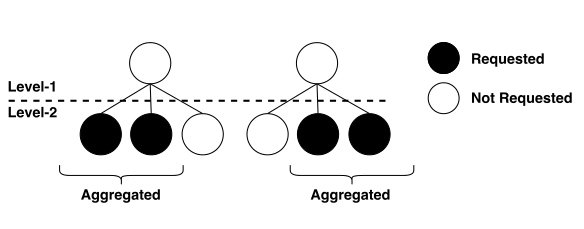
\includegraphics[scale=0.5]{Figs/tree.png}
\caption{A Practical Request Scenario in the Hierarchical Setting}
\label{fig:agg}
\end{figure*}




\subsection{Security of Hierarchical KAC}
\label{subsec:securityhierarchical}

For the CPA security of hierarchical KAC, we state the following theorem.
\begin{Theorem}
\label{th:hierarchicalCPA}
Let $\mathbb{G}_1$ and $\mathbb{G}_2$ be bilinear elliptic curve subgroups of prime order $q$. For any pair of positive integers $n',n (n'>n)$, the hierarchical KAC is $(\tau,\epsilon,n')$ CPA secure if the decision $(\tau,\epsilon,n,n)$-BDHE assumption holds in $(\mathbb{G}_1,\mathbb{G}_2)$.
\end{Theorem}

\noindent Once again, the proof of this theorem is very similar to the proof of Theorem \ref{th:basicCPA} and is hence avoided. Additionally, the hierarchical KAC scheme can also be easily modified to obtain a CCA-secure hierarchical KAC along similar lines to the discussion in Section \ref{sec:CCA}.

\subsection{Owner-Defined Hierarchy}
\label{subsec:owner}

The hierarchical KAC described above fixes the number of hierarchy levels to a pre-defined quantity $K$. This means any path in the hierarchy tree from the root to the length is of length $K+2$. However, in a realistic scenario, it is easy to see that a data owner may want to have her own hierarchical construction and customize the number of levels in the hierarchy. The existing construction of hierarchical KAC can be easily adopted for this scenario by taking either of the following steps:

\begin{itemize}
 \item The system may have a pre-defined upper bound $K$ on the number of hierarchy levels. A data owner willing to go beyond this level must register again with a different set of public, private and access keys to share the additional data classes. A data owner with fewer hierarchy levels than $K$ can have some \emph{dummy nodes} that merely act as placeholders in the overall hierarchy.
 
 \item The other option is to have variable size indexes for different nodes depending on the depth of the hierarchical structure to which it belongs. As and when the hierarchy levels change, the length of index for each node in the hierarchy also changes. This system would require updating the index for each and every data class node in the hierarchy every time a new level is introduced or an old level is deleted. But it does avoid the use of dummy rounds, and allows the data owner the flexibility to increase the number of levels in the hierarchy.
\end{itemize}



\subsection{Advantage over Hierarchical Cryptosystems}
\label{subsec:advantage}


We end this section by pointing out that a major advantage of our proposed hierarchical KAC is that it avoids a significant pitfall of several existing hierarchical encryption based schemes \cite{akl1983cryptographic,ateniese2012provably}. In standard tree based hierarchical systems, granting access to the key corresponding to any node implicitly grants access to all the keys in the subtree rooted at that node. This means granting access to a selected set of nodes in a given subtree would blow up the key-size to be the same as the number of nodes. This is avoided in our two-tier scheme, since decryption rights to any number of nodes (data classes) rooted at a particular node of the hierarchy tree may be aggregated into a single key corresponding to that node. Figure \ref{fig:agg} summarizes this phenomenon for a simple two-level hierarchical system. In the situation depicted, a tree-based hierarchy system would require $4$ constant size decryption keys, while our proposed hierarchical scheme would require only $2$ constant-size decryption keys. The savings is much more pronounced as the number of hierarchy levels increase, as depicted in the following section via simulation studies in practical deployment scenarios.





\section{Conclusions and Future Work}
\label{sec:conclusions}

In this paper, we have proposed a secure and dynamic key aggregate encryption scheme for online data sharing. Our scheme allows data owners to delegate users with access rights to multiple ciphertext classes using a single decryption key that combines the decrypting power of individual keys corresponding to each ciphertext class. Unlike existing key aggregate schemes that are static in their access right delegation policies, our scheme allows data owners to dynamically revoke one or more users' access rights without having to change either the public or the private parameters/keys. The use of bilinear pairings over additive elliptic curve subgroups in our scheme helps achieve massive reductions in key and ciphertext sizes over existing schemes that use multiplicative groups. We pointed out that a possible criticism of this scheme is that the number of classes is pre-defined to some fixed $n$. To deal with this issue, we next proposed a generalized two-level construction of the basic scheme that runs $n_1$ instances of the basic scheme in parallel, with each instance handling key aggregation for $n_2$ ciphertext classes. This scheme provides two major advantages. First of all, it allows dynamic extension of ciphertext classes by registering of new public key-private key pairs without affecting other system parameters. Secondly, it provides a wide range of choices for $n_1$ and $n_2$ that allows efficient utilization of ciphertext classes while also achieving optimum space and time complexities. Finally, we extend the generalized scheme to allow the use of popular and efficiently implementable bilinear pairings in literature such as Tate Pairings that operate on multiple elliptic curve subgroups instead of one. Each of the three proposed schemes have been proven to be semantically secure. Experimental studies have demonstrated the superiority of our proposed scheme over existing ones in terms of key size as well as efficient utilization of ciphertext classes. A possible future work is to make the proposed schemes secure against chosen ciphertext attacks.

\begin{scriptsize}
\bibliographystyle{unsrt}
\bibliography{bib/KeyAggregate}
\end{scriptsize}

% \newpage
% \appendix


% However, KAC suffers from the following major drawbacks:
% 
% \begin{enumerate}
%  \item KAC uses bilinear non-degenerate pairings over multiplicative groups. Recent reports from NIST \cite{NIST2009} have demonstrated that the security of RSA over multiplicative cyclic groups for a key size of $1024$ bits has the same security as RSA over additive elliptic curve groups with a key size of $160$ bits. Thus defining KAC over multiplicative groups is possibly not the most computationally efficient scheme; an adaptation of the scheme to additive elliptic curve group would certainly be more efficient.
%  \item KAC is a static scheme in the sense that once a user is in possession of the aggregate key corresponding to a subset of files from data owner, the owner cannot dynamically revoke the permission of the client for accessing one or more updated files. Since dynamic changes in access rights is extremely common in shared data storage on cloud, this scenario needs to be tackled. 
%  \item The public key extension of KAC proposed in \cite{chu2014key} is extremely cumbersome and resource consuming since registration of each new public key-private key pair requires the number of classes to be extended by th original number of classes.
%  \end{enumerate}

% In this work, we aim to scheme for online data sharing that overcomes to a large extent all of the above mentioned drawbacks of KAC.

% In this paper we aim to present a scheme the above drawbacks of KAC. We also present security proofs for our proposed scheme. We then further extend the scheme using the ideas presented in \cite{} to make it secure against chosen ciphertext attacks.




\section{Bilinear Maps and the BDHE on Elliptic Curves}
\label{app_sec:prelims}

\subsection{Bilinear Pairings}

We  present a brief outline of the necessary facts about bilinear pairings on elliptic curves that are used in the forthcoming discussion. Let $\mathbb{K}=F_{p}$ be a field of prime order $p$, and let an elliptic curve over $\mathbb{K}$ be defined by the Weierstrass \cite{miller1986use} equation:
\begin{equation*}
 E(\mathbb{K}) : y^2 + a_1xy + a_3y = x^3 + a_2x^2 + a_4x + a_6
\end{equation*}

where $a_1, a_2, a_3, a_4, a_5 \in \mathbb{K}$. The curve must be non-singular. In particular, if $char(\mathbb{K})\neq2,3$, the equation takes the special form $y^2=x^3+a_4x+a_6$ with $4{a_4}^3+27{a_6}^2\neq0$. Let $\overline{K} = F_{p^k}$ be the smallest extension field of $K=F_p$ that contains the $q^{th}$ roots of unity. Here, $k$ is called the embedding degree with respect to $K$ and $q$. We denote the set of $q$-torsion points on the elliptic curve as $E(\overline{K})[q]$ ($q$-torsion points essentially have order $q$).

A pairing is a bilinear map defined over elliptic curve subgroups. Let $\mathbb{G}_{1}$ and $\mathbb{G}_{2}$ be two such additive cyclic subgroups of the same prime order $q$ and let $\mathbb{G}_{T}$ be a multiplicative group, also of order $q$ with identity element $1$. Let $P$ and $Q$ be generators for $\mathbb{G}_1$ and $\mathbb{G}_2$ respectively. A pairing $\hat{e'}:\mathbb{G}_1 \times \mathbb{G}_2\longrightarrow\mathbb{G}_T$ satisfying the following the following properties is said to be a bilinear mapping. 

\begin{itemize}
 \item Bilinear: $\forall P_1,P_2 \in \mathbb{G}_1, Q_1,Q_2\in\mathbb{G}_2$, and $a,b \in \mathbb{Z}$, we have the following:
 \begin{eqnarray}
   \hat{e'}(aP_1,bQ_1) &= \hat{e'}(P_1,Q_1)^{ab}\nonumber\\
   \hat{e'}(P_1+P_2,Q_1) &= \hat{e'}(P_1,Q_1)\hat{e'}(P_2,Q_1)\nonumber\\
   \hat{e'}(P_1,Q_1+Q_2) &= \hat{e'}(P_1,Q_1)\hat{e'}(P_1,Q_2)\nonumber
 \end{eqnarray}
 \item Non-degeneracy: If for all $P_i \in \mathbb{G}_1, \hat{e'}(P_1,Q_1)=1$ then $Q_1=\mathcal{0}$. Alternatively, if $P$ and $Q$ be the generators for $\mathbb{G}_1$ and $\mathbb{G}_2$ respectively where neither group only contains the point at infinity, then $\hat{e'}(P,Q)\neq1$ 
 \item Computability: There exists an efficient algorithm to compute $\hat{e'}(R,S)\forall R \in \mathbb{G}_1, S\in\mathbb{G}_2$
\end{itemize}

It is important to note that $\mathbb{G}_1$ and $\mathbb{G}_2$ could be identical groups as well.

% \subsection{The Decisional Bilinear Diffie-Hellman Problem (DBDH)}

% The three-party Diffie-Hellman key agreement \cite{} lends itself to the decisional form - the decisional bilinear Diffie-Hellman (DBDH) problem. DBDH requires a participant to determine if some target element is either a special combination of given parameters or a random element

% Let $\mathbb{G}$ be an additive cyclic elliptic curve subgroup of prime order $q$, where $2^{\lambda}\leq q \leq 2^{\lambda + 1}$, such that the point $P$ is a generator for $\mathbb{G}$. Also, let $\mathbb{G}_{T}$ be a multiplicative group of order $q$ with identity element $1$. We assume that there exists an efficiently computable bilinear pairing $\hat{e'}:\mathbb{G} \times \mathbb{G}\longrightarrow\mathbb{G}_T$. The DBDH problem is defined as follows.  Given $aP, bP, cP \in \mathbb{G}$ where $a,b,c\in \mathbb{Z}_q$, and $T\in \mathbb{G}_T$, determine if $T=\hat{e'}(P,P)^{abc}$. 

% \subsection{The Bilinear Diffie-Hellman Exponent Problem (BDHE)}







\section{Semantic Security of Key-Aggregate Schemes}
\label{app_sec:security}

We now define the semantic security of a key-aggregate encryption system against an adversary using the following game between an attack algorithm $\mathcal{A}$ and a challenger $\mathcal{B}$. Both $\mathcal{A}$ and $\mathcal{B}$ are given $n$, the total number of ciphertext classes, as input. The game proceeds through the following stages.

\begin{enumerate}
 \item \textbf{Init:} Algorithm $\mathcal{A}$ begins by outputting a set $\mathcal{S} \subset \{1,2,\cdots,n\}$ of receivers that it wants to
attack.  For each ciphertext class $i\in\mathcal{S}$, challenger $\mathcal{B}$ performs the \textbf{SetUp}-$\mathbf{i}$, \textbf{Challenge}-$\mathbf{i}$ and \textbf{Guess}-$\mathbf{i}$ steps. Note that the number of iterations is polynomial in $|S|$.

 \item \textbf{SetUp}-$\mathbf{i}$: Challenger $\mathcal{B}$ generates the public $param$, public key $PK$, the access parameter $U$, and provides them to $\mathcal{A}$. In addition, $\mathcal{B}$ also generates and furnishes $\mathcal{A}$ with the aggregate key $K_{\overline{\mathcal{S}}}$ that allows $\mathcal{A}$ to decrypt any ciphertext class $j\notin\mathcal{S}$. 
 \item \textbf{Challenge}-$\mathbf{i}$: Challenger $\mathcal{B}$ performs an encryption of the secret message $m_i$ belonging to the $i^{th}$ class to obtain the ciphertext $\mathcal{C}$. Next, $\mathcal{B}$ picks a random $b\in{(0,1)}$. It sets $T_b = m_i$ and picks a random $T_{1- b}$ from the set of possible plaintext messages. It then gives $(\mathcal{C}, T_0, T_1)$ to algorithm $\mathcal{A}$ as a challenge.

 
 \item\textbf{Guess}-$\mathbf{i}$: The adversary $\mathcal{A}$ outputs a guess $b'$ of $b$. If $b' = b$, $\mathcal{A}$ wins. Otherwise, the game moves on to the next ciphertext class in $\mathcal{S}$ until all ciphertext classes in $\mathcal{S}$ are exhausted.
\end{enumerate}
% \vspace{-2mm}
If $\mathcal{A}$ fails to predict correctly for all ciphertext classes in $\mathcal{S}$, then $\mathcal{A}$ loses the game. Let $AdvKAC_{\mathcal{A},n}$ denote the probability that $\mathcal{A}$ wins the game when the challenger is given $n$ as input. We say that a key-aggregate encryption system is $(\tau,\epsilon,n)$ semantically secure if for all $\tau$-time algorithms $\mathcal{A}$ we have that $|AdvKAC_{\mathcal{A},n}-\frac{1}{2}| < \epsilon$ where $\epsilon$ is a very small quantity. 

The above mentioned game could be looked upon as analogous to a practical attack scenario where users with decryption rights to ciphertext classes not in $\mathcal{S}$, launch a combined attack on $\mathcal{S}$. The adversary $\mathcal{A}$ chooses the subset $\mathcal{S}$ of ciphertext classes she wishes to attack. Note that the adversary $\mathcal{A}$ is non-adaptive; it chooses $\mathcal{S}$, and obtains the aggregate decryption key for all ciphertext classes outside of $\mathcal{S}$, before it even sees the public parameters $param$ or the public key $PK$. An adaptive adversary could request ciphertext classes adaptively. We prove the security of our proposed schemes in the non-adaptive settings described above. We also note that our definition of semantic security for key-aggregate cryptosystems is similar to that for broadcast encryption systems proposed in \cite{boneh2005collusion}.

 

\section{Proof of Correctness of the Generalized Key-Aggregate Encryption Scheme}
\label{app_sec:correct_general}

In this section, we present a proof of correctness for the generalized key-aggregate encryption scheme. Let $\hat{m}$ be the output message produced by decryption corresponding to the plaintext $m$. We assume that the output is not $\bot$. 

\begin{scriptsize}
\begin{equation}
\begin{split}
 \hat{m} &= c_3\frac{\hat{e'}(k^{i_1}_{\mathcal{S}}+\sum_{(i_1,j_2)\in\mathcal{S},j_2\neq i_2}P_{n_2+1-j_2+i_2},U+c_1)}{\hat{e'}(\sum_{(i_1,j_2)\in\mathcal{S}}P_{n_2+1-j_2},c_2)}\\
  &= c_3\frac{\hat{e'}(\sum_{(i_1,j_2)\in \mathcal{S}}{\gamma_{i_1}}P_{n_2+1-j_2} + \sum_{(i_1,j_2)\in\mathcal{S},j_2\neq i_2}P_{n_2+1-j_2+i_2},t'P)}{\hat{e'}(\sum_{(i_1,j_2)\in\mathcal{S}}P_{n_2+1-j_2},t'(pk_{i_1}+P_{i_2})}\\
  &= c_3\frac{\hat{e'}(\sum_{(i_1,j_2)\in \mathcal{S}}{\gamma_{i_1}}P_{n_2+1-j_2},t'P)\hat{e'}(\sum_{(i_1,j_2)\in\mathcal{S}}(P_{n_2+1-j_2+i_2})-P_{n_2+1},t'P)}{\hat{e'}(\sum_{(i_1,j_2)\in\mathcal{S}}P_{n_2+1-j_2},t'pk_{i_1})\hat{e'}(\sum_{(i_1,j_2)\in\mathcal{S}}P_{n_2+1-j_2},t'P_{i_2})}\\
  &= c_3\frac{\hat{e'}(\sum_{(i_1,j_2)\in\mathcal{S}}P_{n_2+1-j_2+i_2},t'P)}{\hat{e'}(P_{n_2+1},t'P)\hat{e'}(\sum_{(i_1,j_2)\in\mathcal{S}}P_{n_2+1-j_2},t'P_{i_2})}\\
  &= c_3\frac{\hat{e'}(\sum_{(i_1,j_2)\in\mathcal{S}}P_{n_2+1-j_2+i_2},t'P)}{\hat{e'}(P_{n_2+1},t'P)\hat{e'}(\sum_{(i_1,j_2)\in\mathcal{S}}P_{n_2+1-j_2+i_2},t'P)}\\
  &= m\frac{\hat{e'}(P_{n_2},t'P_1)}{\hat{e'}(P_{n_2+1},t'P)}\\
  &= m
\end{split}  
\end{equation}
\end{scriptsize}


\section{Proof of Semantic Security of the Generalized Key-Aggregate Encryption Scheme}
\label{app_sec:proof_general}

\subsection{The Reduced Generalized Scheme}

As in the original scheme, we may analogously define a reduced version of the generalized encryption scheme. We note that once again, in the generalized scheme, the ciphertext $\mathcal{C}=(c_1,c_2,c_3)$ output by the $Encypt$ operation essentially embeds the value of $m$ in $c_3$ by multiplying it with $\hat{e'}(P_{n_2},tP_1)$. Consequently, the security of our proposed scheme is equivalent to that of a \emph{reduced} generalized key-aggregate encryption scheme that simply uses the reduced ciphertext $(c_1,c_2)$, the aggregate key $K_{\mathcal{S}}$ and the dynamic access parameter $U$ to successfully transmit and decrypt the value of $\hat{e'}(P_{n_2},t'P_1)=\hat{e'}(P_{n_2+1},t'P)$. We prove the semantic security of this \emph{reduced scheme} parameterized with a given number of ciphertext classes $n_2$ for each instance, which also amounts to proving the semantic security of our original encryption scheme for the same number of ciphertext classes. Note that the proof of security is independent of the 
number of instances $n_1$ that run in parallel.

\subsection{The Adversarial Model} We make the following assumptions about the adversary $\mathcal{A}$:

\begin{enumerate}
 \item The adversary has the aggregate key that allows her to access any ciphertext class other than those in the target subset $\mathcal{S}$, that is, she possesses $K_{\overline{\mathcal{S}}}$.
 \item The adversary has access to the public parameters $param$ and $PK$, and also possesses the dynamic access parameter $U$.
%  \item The adversary is authorized and and hence 
\end{enumerate}


\subsection{The Security Proof}

The security proof presented here uses the first complexity assumption stated in \ref{subsubsec:asm_1}. Let $\mathbb{G}$ be a bilinear elliptic curve subgroup of prime order $q$ and $G_T$ be a multiplicative group of order $q$. Let $\hat{e'}:\mathbb{G} \times \mathbb{G}\longrightarrow\mathbb{G}_T$ be a bilinear non-degenerate pairing. For any pair of positive integers $n_2,n' (n'>n_2)$ our proposed $n_2$-generalized reduced key-aggregate encryption scheme over elliptic curve subgroups is $(\tau,\epsilon,n')$ semantically secure if the decision $(\tau,\epsilon,n_2)$-BDHE assumption holds in $\mathbb{G}$. We now prove this statement below.

\textbf{\noindent{Proof:}} Let for a given input $n'$, $\mathcal{A}$ be a $\tau$-time adversary that has advantage greater than $\epsilon$ for the \emph{reduced scheme} parameterized with a given $n_2$. We build an algorithm $\mathcal{B}$ that has advantage at least $\epsilon$ in solving the $n_2$-BDHE problem in $\mathbb{G}$. Algorithm $\mathcal{B}$ takes as input a random $n_2$-BDHE challenge $(P,H,Y_{(P,\alpha,n_2)},Z)$ where $Z$ is either $\hat{e'}(P_{n_2+1},H)$ or a random value in $\mathbb{G}_T$. Algorithm $\mathcal{B}$ proceeds as follows.

\begin{enumerate}
 \item \textbf{Init:} Algorithm $\mathcal{B}$ runs $\mathcal{A}$ and receives the set $\mathcal{S}$ of ciphertext classes that $\mathcal{A}$ wishes to be challenged on. For each ciphertext class $(i_1,i_2)\in\mathcal{S}$, $\mathcal{B}$ performs the \textbf{SetUp}-$\mathbf{(i_1,i_2)}$, \textbf{Challenge}-$\mathbf{(i_1,i_2)}$ and \textbf{Guess}-$\mathbf{(i_1,i_2)}$ steps. Note that the number of iterations is polynomial in $|S|$. 
 
 \item \textbf{SetUp}-$\mathbf{(i_1,i_2)}$: $\mathcal{B}$ should generate the public $param$, public key $PK$, the access parameter $U$, and the aggregate key $K_{\overline{\mathcal{S}}}$. For the iteration corresponding to ciphertext class $(i_1,i_2)$, they are generated as follows.
 \begin{itemize}
  \item $param$ is set as $(P,Y_{P,\alpha,n_2})$.
  \item Randomly generate $u_1,u_2,\cdots,u_{n_1} \in \mathbb{Z}_q$. Then, set\\ $PK$=$(pk_1,pk_2,\cdots,pk_{n_1})$, where $pk_{j_1}$ is set as $u_{j_1}P - P_{i_2}$ for $j_1=1,2,\cdots,n_1$.
  \item $K_{\overline{\mathcal{S}}}$ is set as $(k^{1}_{\overline{\mathcal{S}}},k^{2}_{\overline{\mathcal{S}}},\cdots,k^{n_1}_{\overline{\mathcal{S}}})$ where $k^{j_1}_{\overline{\mathcal{S}}}$ = $\sum_{(j_1,j_2)\notin\mathcal{S}}({u}P_{n_2+1-j_2}-(P_{n_2+1-j_2+i_2}))$ for $j_1=1,2,\cdots,n_1$. Note that this implies $k^{j_1}_{\overline{\mathcal{S}}}$ is equal to $\sum_{(j_1,j_2)\notin\mathcal{S}}\alpha^{n_2+1-j_2}pk_{j_1}$, as is supposed to be as per the scheme specification. Note that $\mathcal{B}$ knows that $(i_1,i_2)\notin \overline{\mathcal{S}}$, and hence has all the resources to compute this aggregate key for $\overline{\mathcal{S}}$. 
  \item $U$ is set as some random element in $\mathbb{G}$.
 \end{itemize}
 
 Note that since $P$, $\alpha$, $U$ and the $u_{j_1}$ values are chosen uniformly at random, the public key has an identical distribution to that in the actual construction.
 
 \item \textbf{Challenge}-$\mathbf{(i_1,i_2)}$: To generate the challenge for the ciphertext class $(i_1,i_2)$, $\mathcal{B}$ computes $(c_1,c_2)$ as $(H-U,u_{i_1}H)$. It then randomly chooses a bit $b\in{(0,1)}$ and sets $T_b$ as $Z$ and $T_{1-b}$ as a random element in $\mathbb{G}_T$. The challenge given to $\mathcal{A}$ is $((c_1,c_2),T_0,T_1)$. 
 
 We claim that when $Z=\hat{e'}(P_{n_2+1},H)$ (i.e. the input to $\mathcal{B}$ is a $n_2$-BDHE tuple), then $((c_1,c_2),T_0,T_1)$ is a valid challenge to $A$. We prove this claim here. we point out that $P$ is a generator of $\mathbb{G}$ and so $H=t'P$ for some $t'\in\mathbb{Z}_q$. Putting $H$ as $t'P$ gives us the following:
 \begin{itemize}
  \item  $U=tP$ for some $t\in\mathbb{Z}_q$
  \item $c_1=H-U=(t'-t)P=rP$ for $r=t'-t$
  \item $c_2=u_{i_1}H=(u_{i_1})t'P=t'(u_{i_1}P)=t'(u_{i_1}P-P_{i_2}+P_{i_2})=t'(pk_{i_1}+P_{i_2})$
  \item $K_b=Z=\hat{e'}(P_{n_2+1},H)=\hat{e'}(P_{n_2+1},t'P)$
 \end{itemize}
 On the other hand, if $Z$ is a random element in $\mathbb{G}_T$ (i.e. the input to $\mathcal{B}$ is a random tuple), then $K_0$ and $K_1$ are just random independent elements of $\mathbb{G}_T$.
 
 \item\textbf{Guess}-$\mathbf{(i_1,i_2)}$: The adversary $\mathcal{A}$ outputs a guess $b'$ of $b$. If $b' = b$, $\mathcal{B}$ outputs $0$ (indicating that $Z = \hat{e'}(P_{n+1},H)$), and terminates. Otherwise, it goes for the next ciphertext class in $\mathcal{S}$.
\end{enumerate}
If after $|\mathcal{S}|$ iterations, $b' \neq b$ for each ciphertext class $(i_1,i_2)\in\mathcal{S}$, the algorithm $\mathcal{B}$ outputs $0$ (indicating that $Z = \hat{e'}(P_{n_2+1},H)$). Otherwise, it outputs $1$ (indicating that $Z$ is random in $\mathbb{G}_T$). We now analyze the probability that $\mathcal{B}$ gives a correct output. If $(P,H,Y_{(P,\alpha,n_2)},Z)$ is sampled from $R$-BDHE, $Pr[\mathcal{B}(G,H,Y_{(P,\alpha,n_2)},Z)=0]$ = $\frac{1}{2}$, while if $(P,H,Y_{(P,\alpha,n_2)},Z)$ is sampled from $L$-BDHE, $|Pr[\mathcal{B}(G,H,Y_{(P,\alpha,n_2)},Z)]-\frac{1}{2}|$ $\geq$ $\epsilon$. So, the probability that $\mathcal{B}$ outputs correctly is at least $1-(\frac{1}{2}-\epsilon)^{|\mathcal{S}|} \geq \frac{1}{2}+\epsilon$. Thus $\mathcal{B}$ has advantage at least $\epsilon$ in solving the $n_2$-BDHE problem. This concludes the proof.


\section{Proof of Correctness of the Extended Key-Aggregate Encryption Scheme:}
\label{app_sec:correct_extended}

In this section, we present a proof of correctness for the extended key-aggregate encryption scheme. Let $\hat{m}$ be the output message produced by decryption corresponding to the plaintext $m$. We assume that the output is not $\bot$. 

\begin{scriptsize}
\begin{equation}
\begin{split}
 \hat{m} &= c_3\frac{\hat{e''}(k^{i_1}_{\mathcal{S}}+\sum_{(i_1,j_2)\in\mathcal{S},j_2\neq i_2}P_{n_2+1-j_2+i_2},U+c_1)}{\hat{e''}(\sum_{(i_1,j_2)\in\mathcal{S}}P_{n_2+1-j_2},c_2)}\\
  &= c_3\frac{\hat{e''}(\sum_{(i_1,j_2)\in \mathcal{S}}{\gamma_{i_1}}P_{n_2+1-j_2} + \sum_{(i_1,j_2)\in\mathcal{S},j_2\neq i_2}P_{n_2+1-j_2+i_2},t'Q)}{\hat{e''}(\sum_{(i_1,j_2)\in\mathcal{S}}P_{n_2+1-j_2},t'({pk^2}_{i_1}+Q_{i_2}))}\\
  &= c_3\frac{\hat{e''}(\sum_{(i_1,j_2)\in \mathcal{S}}{\gamma_{i_1}}P_{n_2+1-j_2},t'Q)\hat{e''}(\sum_{(i_1,j_2)\in\mathcal{S}}(P_{n_2+1-j_2+i_2})-P_{n_2+1},t'Q)}{\hat{e''}(\sum_{(i_1,j_2)\in\mathcal{S}}P_{n_2+1-j_2},\gamma_{i_1}(t'Q))\hat{e''}(\sum_{(i_1,j_2)\in\mathcal{S}}P_{n_2+1-j_2},\alpha^{i_2}(t'Q))}\\
  &= c_3\frac{\hat{e''}(\sum_{(i_1,j_2)\in\mathcal{S}}P_{n_2+1-j_2+i_2},t'Q)}{\hat{e''}(P_{n_2+1},t'Q)\hat{e''}(\sum_{(i_1,j_2)\in\mathcal{S}}P_{n_2+1-j_2},\alpha^{i_2}(t'Q))}\\
  &= c_3\frac{\hat{e''}(\sum_{(i_1,j_2)\in\mathcal{S}}P_{n_2+1-j_2+i_2},t'Q)}{\hat{e''}(P_{n_2+1},t'Q)\hat{e''}(\sum_{(i_1,j_2)\in\mathcal{S}}P_{n_2+1-j_2+i_2},t'Q)}\\
  &= m\frac{\hat{e''}(P_{n_2},t'Q_1)}{\hat{e''}(P_{n_2+1},t'Q)}\\
  &= m
\end{split}  
\end{equation}
\end{scriptsize}

\section{Proof of Semantic Security of the Extended Key-Aggregate Encryption Scheme}
\label{app_sec:proof_extended}

\subsection{The Reduced Version of the Extended Key-Aggregate Scheme}

As in the earlier schemes, we define a reduced version of the extension to the generalized encryption scheme. The security of our proposed extended scheme is equivalent to that of a \emph{reduced} scheme that simply uses the reduced ciphertext $(c_1,c_2)$, the aggregate key $K_{\mathcal{S}}$ and the dynamic access parameter $U$ to successfully transmit and decrypt the value of $\hat{e'}(P_{n_2},t'Q_1)=\hat{e'}(P_{n_2+1},t'Q)$. We prove the semantic security of this \emph{reduced scheme} parameterized with a given number of ciphertext classes $n_2$ for each instance, which also amounts to proving the semantic security of our original encryption scheme for the same number of ciphertext classes. Note that the proof of security is independent of the number of instances $n_1$ that run in parallel.

\subsection{The Adversarial Model} We make the following assumptions about the adversary $\mathcal{A}$:

\begin{enumerate}
 \item The adversary has the aggregate key that allows her to access any ciphertext class other than those in the target subset $\mathcal{S}$, that is, she possesses $K_{\overline{\mathcal{S}}}$.
 \item The adversary has access to the public parameters $param$, $PK^1$ and $PK^2$, and also possesses the dynamic access parameter $U$.
%  \item The adversary is authorized and and hence 
\end{enumerate}


\subsection{The Security Proof}

The security proof presented here uses the second complexity assumption stated in \ref{subsubsec:asm_2}. Let $\mathbb{G_1}$ and $\mathbb{G}_2$ be additive elliptic curve subgroups of prime order $q$, and $G_T$ be a multiplicative group of order $q$. Let $\hat{e''}:\mathbb{G}_1 \times \mathbb{G}_2\longrightarrow\mathbb{G}_T$ be a bilinear non-degenerate pairing. We claim that for any pair of positive integers $n_2,n' (n'>n_2)$ our proposed extension to the $n_2$-generalized reduced key-aggregate encryption scheme over elliptic curve subgroups is $(\tau,\epsilon,n')$ semantically secure if the decision $(\tau,\epsilon,n_2,n_2)$-BDHE assumption holds in $(\mathbb{G}_1,\mathbb{G}_2)$. \textbf{As already proved in Appendix \ref{app_sec:hardness}, the decision $(\tau,\epsilon,l,l)$-BDHE assumption for elliptic curves holds in equi-prime order subgroups $(\mathbb{G}_1,\mathbb{G}_2)$ if the decision $(\tau,\epsilon,l)$-BDHE assumption for elliptic curves holds in $\mathbb{G}_1$}. Thus proving the aforementioned 
claim amounts to proving that our proposed extension to the $n_2$-generalized reduced key-aggregate encryption scheme over elliptic curve subgroups is $(\tau,\epsilon,n')$ semantically secure if the decision $(\tau,\epsilon,l)$-BDHE assumption for elliptic curves holds in $\mathbb{G}_1$. We now prove the claim below.

\textbf{\noindent{Proof:}} Let for a given input $n'$, $\mathcal{A}$ be a $\tau$-time adversary that has advantage greater than $\epsilon$ for the \emph{reduced scheme} parameterized with a given $n_2$. We build an algorithm $\mathcal{B}$ that has advantage at least $\epsilon$ in solving the $(n_2,n_2)$-BDHE problem in $\mathbb{G}$. Algorithm $\mathcal{B}$ takes as input a random $(n_2,n_2)$-BDHE challenge $(P,Q,H,Y_{(P,\alpha,n_2),Y'_{Q,\alpha,n_2}},Z)$ where $Z$ is either $\hat{e''}(P_{n_2+1},H)$ or a random value in $\mathbb{G}_T$. Algorithm $\mathcal{B}$ proceeds as follows.

\begin{enumerate}
 \item \textbf{Init:} Algorithm $\mathcal{B}$ runs $\mathcal{A}$ and receives the set $\mathcal{S}$ of ciphertext classes that $\mathcal{A}$ wishes to be challenged on. For each ciphertext class $(i_1,i_2)\in\mathcal{S}$, $\mathcal{B}$ performs the \textbf{SetUp}-$\mathbf{(i_1,i_2)}$, \textbf{Challenge}-$\mathbf{(i_1,i_2)}$ and \textbf{Guess}-$\mathbf{(i_1,i_2)}$ steps. Note that the number of iterations is polynomial in $|S|$. 
 
 \item \textbf{SetUp}-$\mathbf{(i_1,i_2)}$: $\mathcal{B}$ should generate the public $param$, public keys $PK^1,PK^2$, the access parameter $U$, and the aggregate key $K_{\overline{\mathcal{S}}}$. For the iteration corresponding to ciphertext class $(i_1,i_2)$, they are generated as follows.
 \begin{itemize}
  \item $param$ is set as $(P,Q,Y_{P,\alpha,n_2},Y'_{Q,\alpha,n_2})$.
  \item Randomly generate $u_1,u_2,\cdots,u_{n_1} \in \mathbb{Z}_q$. Then, set\\ $PK^1$=$({pk^1}_1,{pk^1}_2,\cdots,{pk^1}_{n_1})$, where ${pk^1}_{j_1}$ is set as $u_{j_1}P - P_{i_2}$ for $j_1=1,2,\cdots,n_1$, and set\\ $PK^2$=$({pk^2}_1,{pk^2}_2,\cdots,{pk^2}_{n_1})$, where ${pk^2}_{j_1}$ is set as $u_{j_1}Q - Q_{i_2}$ for $j_1=1,2,\cdots,n_1$
  \item $K_{\overline{\mathcal{S}}}$ is set as $(k^{1}_{\overline{\mathcal{S}}},k^{2}_{\overline{\mathcal{S}}},\cdots,k^{n_1}_{\overline{\mathcal{S}}})$ where $k^{j_1}_{\overline{\mathcal{S}}}$ = $\sum_{(j_1,j_2)\notin\mathcal{S}}({u}P_{n_2+1-j_2}-(P_{n_2+1-j_2+i_2}))$ for $j_1=1,2,\cdots,n_1$. Note that this implies $k^{j_1}_{\overline{\mathcal{S}}}$ is equal to $\sum_{(j_1,j_2)\notin\mathcal{S}}\alpha^{n_2+1-j_2}{pk^{1}}_{j_1}$, as is supposed to be as per the scheme specification. Note that $\mathcal{B}$ knows that $(i_1,i_2)\notin \overline{\mathcal{S}}$, and hence has all the resources to compute this aggregate key for $\overline{\mathcal{S}}$. 
  \item $U$ is set as some random element in $\mathbb{G}_2$.
 \end{itemize}
 
 Note that since $P$, $Q$, $\alpha$, $U$ and the $u_{j_1}$ values are chosen uniformly at random, the public key has an identical distribution to that in the actual construction.
 
 \item \textbf{Challenge}-$\mathbf{(i_1,i_2)}$: To generate the challenge for the ciphertext class $(i_1,i_2)$, $\mathcal{B}$ computes $(c_1,c_2)$ as $(H-U,u_{i_1}H)$. It then randomly chooses a bit $b\in{(0,1)}$ and sets $T_b$ as $Z$ and $T_{1-b}$ as a random element in $\mathbb{G}_T$. The challenge given to $\mathcal{A}$ is $((c_1,c_2),T_0,T_1)$. 
 
 We claim that when $Z=\hat{e''}(P_{n_2+1},H)$ (i.e. the input to $\mathcal{B}$ is a $n_2$-BDHE tuple), then $((c_1,c_2),T_0,T_1)$ is a valid challenge to $A$. We prove this claim here. we point out that $Q$ is a generator of $\mathbb{G}_2$ and so $H=t'P$ for some $t'\in\mathbb{Z}_q$. Putting $H$ as $t'Q$ gives us the following:
 \begin{itemize}
  \item  $U=tQ$ for some $t\in\mathbb{Z}_q$
  \item $c_1=H-U=(t'-t)Q=rQ$ where $r=t'-t$
  \item $c_2=u_{i_1}H=(u_{i_1})t'Q=t'(u_{i_1}Q)=t'(u_{i_1}Q-Q_{i_2}+Q_{i_2})=t'({pk^2}_{i_1}+Q_{i_2})$
  \item $K_b=Z=\hat{e'}(P_{n_2+1},H)=\hat{e'}(P_{n_2+1},t'Q)$
 \end{itemize}
 On the other hand, if $Z$ is a random element in $\mathbb{G}_T$ (i.e. the input to $\mathcal{B}$ is a random tuple), then $K_0$ and $K_1$ are just random independent elements of $\mathbb{G}_T$.
 
 \item\textbf{Guess}-$\mathbf{(i_1,i_2)}$: The adversary $\mathcal{A}$ outputs a guess $b'$ of $b$. If $b' = b$, $\mathcal{B}$ outputs $0$ (indicating that $Z = \hat{e''}(P_{n+1},H)$), and terminates. Otherwise, it goes for the next ciphertext class in $\mathcal{S}$.
\end{enumerate}
If after $|\mathcal{S}|$ iterations, $b' \neq b$ for each ciphertext class $(i_1,i_2)\in\mathcal{S}$, the algorithm $\mathcal{B}$ outputs $0$ (indicating that $Z = \hat{e'}(P_{n_2+1},H)$). Otherwise, it outputs $1$ (indicating that $Z$ is random in $\mathbb{G}_T$). We now analyze the probability that $\mathcal{B}$ gives a correct output. If $(P,H,Y_{(P,\alpha,n_2)},Z)$ is sampled from $R'$-BDHE, $Pr[\mathcal{B}(G,H,Y_{(P,\alpha,n_2)},Z)=0]$ = $\frac{1}{2}$, while if $(P,H,Y_{(P,\alpha,n_2)},Z)$ is sampled from $L'$-BDHE, $|Pr[\mathcal{B}(G,H,Y_{(P,\alpha,n_2)},Z)]-\frac{1}{2}|$ $\geq$ $\epsilon$. So, the probability that $\mathcal{B}$ outputs correctly is at least $1-(\frac{1}{2}-\epsilon)^{|\mathcal{S}|} \geq \frac{1}{2}+\epsilon$. Thus $\mathcal{B}$ has advantage at least $\epsilon$ in solving the $(n_2,n_2)$-BDHE problem. This concludes the proof.

\section{Implementation of Tate pairings Using BN Curves}
\label{app_sec:implementation}

\subsection{The Tate pairing}
% \label{app_subsec:tate}

We first provide a brief overview of the Tate pairing. Let $\mathbb{K}$ be a field of prime order $p$, and let an elliptic curve $E(K)$ over $\mathbb{K}$ be defined by the Weierstrass \cite{miller1986use} equation. Also, Let $\overline{K} = F_{p^k}$ be the smallest extension field of $K=F_p$ that contains the $q^{th}$ roots of unity. We refer to $k$ as the embedding degree with respect to $K$ and $q$. Further, we refer to the set of $q$-torsion points on the elliptic curve as $E(\overline{K})[q]$ ($q$-torsion points essentially have order $q$). Before defining the Tate pairing, we briefly state the Miller's function \cite{miller1986use}. Let $[a]P$ denote the multiplication of a point $P \in E$ by a scalar $a \in \mathbb{Z}$ (equivalent to adding $P$ $a$ times), and let $\mathcal{O} \in E$ denote the point at infinity. A Miller function is any rational function on $E$ that has a divisor of the form
  \begin{equation}
   (f_{q,P}) = q(P)-([q]P)-(q-1)\mathcal{O}.
  \end{equation}
A Miller function has $q$ zeros at $P$, one pole at $[q]P$ and $q-1$ poles at $\mathcal{O}$. For every point $Q\neq P, [q]P, \mathcal{0}$, we have $(f_{q,P})\in {\overline{K}}^{*}$. We now define the Tate pairing over elliptic curves. 

The Tate pairing $e_{T}:\mathbb{G}_1\times \mathbb{G}_2\longrightarrow \mathbb{G}_T$ is a well-defined, non-degenerate, bilinear pairing with $\mathbb{G}_1 = E(K)[q]$, $\mathbb{G}_2=E(\overline{K})/qE(\overline{K})$, and $\mathbb{G}_T = {\overline{K}}^*/({\overline{K}}^{*})^q$. Let $P \in E(\overline{K})[q]$ and $Q \in E(\overline{K})/qE(\overline{K})$. Then the Tate pairing of $P,Q$ is computed as 
\begin{equation}
 e_T(P,Q)=f_{q,P}(Q)^{\frac{p^k-1}{q}}
\end{equation}


\subsubsection{Properties:}
% \label{tate_pairing_properties}
Tate pairing satisfies following properties that make the pairing suitable for use in cryptography.
\begin{itemize}
% [font=$\bullet$]
 \item Well defined:  $e_T(\mathcal{O},Q) =  1$ for all $Q \in E(\overline{K})$ and $e_T(P,Q) \in (\overline{K}^*)^q$ for all $P \in E(\overline{K})[q]$ and all $Q \in qE(\overline{K})$.
 \item Bilinearity: For all $P, P_1, P_2 \in E(\overline{K})[q]$ and $Q, Q_1, Q_2 \in E(\overline{K})$, we have
 \subitem $e_T(P_1+P_2,Q) = e_T(P_1,Q) \cdot e_T(P_2,Q)$.
 \subitem $e_T(P,Q_1+Q_2) = e_T(P,Q_1) \cdot e_T(P,Q_2)$.
 \item Non-degeneracy: For each point $E(\overline{K})[q] \backslash {\mathcal{O}}$ there is some point $Q \in E(\overline{K})$ such that $e_T(P,Q) \notin (\overline{K})^q$.
\end{itemize}

\subsection{Pairing Friendly Curves}

% \section{Barreto-Naehrig Curves}
% \label{bn}
Barreto and Naehrig \cite{barreto2006pairing} developed a method for constructing a method for constructing pairing-friendly elliptic curves over prime fields, with prime order and embedding degree $k = 12$. The equation of the curve is $E : y^2 = x^3 + b$, with $b \neq 0$. The trace (of Frobenius) of the curve, the curve order and the characteristic of $\mathbb{F}_p$  are parameterized as:
\begin{align*}
t(x) &= 6x^2 + 1\\
n(x) &= 36x^4-36x^3+18x^2-6x+1\\
p(x) &= 36x^4-36x^3+24x^2-6x+1\\
\end{align*}
respectively. Such a curve is often referred to in literature a Barreto-Naehrig or BN curve. Since every point on the BN curve has order $n$, the value of $q$ (a large prime dividing the curve order) can be taken to be the same as $n$.

\subsubsection{Suitability of Barreto-Naehrig curves:}
BN curves are especially well suited for the $128$-bit security level. This is because, if $p$ is 256-bit prime, then the Pollard’s rho method for computing discrete logarithms in $E(\mathbb{F}_p)$ has running time approximately $2^{128}$, as does the number field sieve algorithm for computing discrete logarithms in the extension field $\mathbb{F}_{p^{12}}$. The biggest advantage of using BN curves is that they admit \emph{sextic twists} with degree six, implying that there exists a distortion map between $\mathbb{F}_{p^2}$ and $\mathbb{F}_{p^12}$. This is of great advantage from the computational point of view since many computations can now be restricted to the field $\mathbb{F}_{p^2}$. The other advantage of using BN curves is their flexibility in terms of order of the prime $p$.  Barreto and Naehrig have defined in \cite{barreto2006pairing} a whole family of BN curves to choose from, corresponding to primes of any given order.  
\subsubsection{Barreto-Naehrig curve used in implementation}
The BN curve used in our implementation for $256$ bit primes is given by 
\begin{equation}
E : Y^2 = X^3 + 3
\end{equation}
with BN parameter $x = 6000000000001F2D$ (in hexadecimal). The corresponding prime $p(x) = 36x^4-36x^3+24x^2-6x+1$ is a 256-bit prime of Hamming weight 87, $n(x) = 36x^4-36x^3+18x^2-6x+1$ is 256-bit prime of Hamming weight 91, and $t-1 = p-r = 6z^2+1$ is a 128-bit integer of Hamming weight 28(here $t = p+1-r$ is the trace of $E$). Note that the choice of $p$ is made such that $p\equiv{7(mod8)}$, $p\equiv{4(mod9)}$ $p\equiv{1(mod6)}$. The reason for this is as follows.

\begin{enumerate}
 \item The first condition ensures that $-2$ is a quadratic non-residue.
 \item The second condition ensures efficient computation of cube roots \cite{cryptoeprint:2005:133}.
 \item The third condition ensures that there exists $\xi \in \mathbb{F}_{p^2}$ such that $W^6 - \xi$ is irreducible over $\mathbb{F}_{p^2}[W]$.  
 
\end{enumerate}


\subsection{The Finite Field Extensions}

As per the proposition in \cite{devegili2007implementing}, we construct the extension field $\mathbb{F}_{p^{12}}$ using the following tower field extensions: 
\begin{enumerate}
 \item $\mathbb{F}_{p^2} = \mathbb{F}_p[u]/(u^2+2)$,
 \item $\mathbb{F}_{p^6} =\mathbb{F}_{p^2}[v]/(v^3-\xi)$ where $\xi =-u-1$, and
 \item $\mathbb{F}_{p^{12}}=\mathbb{F}_{p^6}[w]/(w^2-v)$.
\end{enumerate}

The quadratic/cubic non-residues and reduction polynomials are detailed in Table \ref{table:field_extensions} for $a_0,a_1\in \mathbb{F}_{p}$, $b_0,b_1,b_2\in\mathbb{F}_{p^2}$, and $c_0,c_1\in\mathbb{F}_{p^6}$.
\begin{table}[h!]
\captionsetup{font=scriptsize}
\caption{Extension fields}
\centering
\label{table:field_extensions}
\begin{tabular}{|c|c|c|c|}
\hline
Extension & Non-Residue & Construction & Representation \\
\hline
$\mathbb{F}_{p^2}$ & $\beta$ = -2 & $\mathbb{F}_p$[$X$]/($X^2$ - $\beta$) & $a$= $a_0$ + $a_1X$ \\
$\mathbb{F}_{p^6}$ & $\xi$ = -1-$\sqrt[]\beta$ & $\mathbb{F}_{p^2}$[$Y$]/($Y^3$ - $\xi$) & $b$= $b_0$ + $b_1Y$ + $b_2Y^2$ \\
$\mathbb{F}_{p^{12}}$ & $\xi'$ = $\sqrt[3]\xi$ & $\mathbb{F}_{p^6}$[$Z$]/($Z^2$ - $\xi'$) & $c$= $c_0$ + $c_1Z$ \\
\hline
\end{tabular}
\end{table}

\subsection{The Actual Implementation}

The computation of the Tate pairing can be broadly divided into two major parts - the Miller's algorithm and the final exponentiation. A detailed  implementation of the Miller's algorithm has been presented in \cite{ghosh2013secure} and we use the same for our experiments. The final exponentiation can also be efficiently implemented using the following factorization.

\begin{align*}
 f^{\frac{p^{12}-1}{q}} &= f^{(p^6-1)\cdot\frac{p^6+1}{p^4-p^2+1}\cdot\frac{p^4-p^2+1}{q}}\\
 &=((f^{p^6-1})^{p^2+1})^\frac{p^4-p^2+1}{q}
\end{align*}



% end{align*}



\end{document}
